% Options for packages loaded elsewhere
\PassOptionsToPackage{unicode}{hyperref}
\PassOptionsToPackage{hyphens}{url}
\PassOptionsToPackage{dvipsnames,svgnames,x11names}{xcolor}
%
\documentclass[
  authoryear,
  review]{elsarticle}

\usepackage{amsmath,amssymb}
\usepackage{iftex}
\ifPDFTeX
  \usepackage[T1]{fontenc}
  \usepackage[utf8]{inputenc}
  \usepackage{textcomp} % provide euro and other symbols
\else % if luatex or xetex
  \usepackage{unicode-math}
  \defaultfontfeatures{Scale=MatchLowercase}
  \defaultfontfeatures[\rmfamily]{Ligatures=TeX,Scale=1}
\fi
\usepackage{lmodern}
\ifPDFTeX\else  
    % xetex/luatex font selection
\fi
% Use upquote if available, for straight quotes in verbatim environments
\IfFileExists{upquote.sty}{\usepackage{upquote}}{}
\IfFileExists{microtype.sty}{% use microtype if available
  \usepackage[]{microtype}
  \UseMicrotypeSet[protrusion]{basicmath} % disable protrusion for tt fonts
}{}
\makeatletter
\@ifundefined{KOMAClassName}{% if non-KOMA class
  \IfFileExists{parskip.sty}{%
    \usepackage{parskip}
  }{% else
    \setlength{\parindent}{0pt}
    \setlength{\parskip}{6pt plus 2pt minus 1pt}}
}{% if KOMA class
  \KOMAoptions{parskip=half}}
\makeatother
\usepackage{xcolor}
\setlength{\emergencystretch}{3em} % prevent overfull lines
\setcounter{secnumdepth}{5}
% Make \paragraph and \subparagraph free-standing
\makeatletter
\ifx\paragraph\undefined\else
  \let\oldparagraph\paragraph
  \renewcommand{\paragraph}{
    \@ifstar
      \xxxParagraphStar
      \xxxParagraphNoStar
  }
  \newcommand{\xxxParagraphStar}[1]{\oldparagraph*{#1}\mbox{}}
  \newcommand{\xxxParagraphNoStar}[1]{\oldparagraph{#1}\mbox{}}
\fi
\ifx\subparagraph\undefined\else
  \let\oldsubparagraph\subparagraph
  \renewcommand{\subparagraph}{
    \@ifstar
      \xxxSubParagraphStar
      \xxxSubParagraphNoStar
  }
  \newcommand{\xxxSubParagraphStar}[1]{\oldsubparagraph*{#1}\mbox{}}
  \newcommand{\xxxSubParagraphNoStar}[1]{\oldsubparagraph{#1}\mbox{}}
\fi
\makeatother


\providecommand{\tightlist}{%
  \setlength{\itemsep}{0pt}\setlength{\parskip}{0pt}}\usepackage{longtable,booktabs,array}
\usepackage{calc} % for calculating minipage widths
% Correct order of tables after \paragraph or \subparagraph
\usepackage{etoolbox}
\makeatletter
\patchcmd\longtable{\par}{\if@noskipsec\mbox{}\fi\par}{}{}
\makeatother
% Allow footnotes in longtable head/foot
\IfFileExists{footnotehyper.sty}{\usepackage{footnotehyper}}{\usepackage{footnote}}
\makesavenoteenv{longtable}
\usepackage{graphicx}
\makeatletter
\newsavebox\pandoc@box
\newcommand*\pandocbounded[1]{% scales image to fit in text height/width
  \sbox\pandoc@box{#1}%
  \Gscale@div\@tempa{\textheight}{\dimexpr\ht\pandoc@box+\dp\pandoc@box\relax}%
  \Gscale@div\@tempb{\linewidth}{\wd\pandoc@box}%
  \ifdim\@tempb\p@<\@tempa\p@\let\@tempa\@tempb\fi% select the smaller of both
  \ifdim\@tempa\p@<\p@\scalebox{\@tempa}{\usebox\pandoc@box}%
  \else\usebox{\pandoc@box}%
  \fi%
}
% Set default figure placement to htbp
\def\fps@figure{htbp}
\makeatother

\usepackage{fontspec}
\usepackage{multirow}
\usepackage{multicol}
\usepackage{colortbl}
\usepackage{hhline}
\newlength\Oldarrayrulewidth
\newlength\Oldtabcolsep
\usepackage{longtable}
\usepackage{array}
\usepackage{hyperref}
\usepackage{float}
\usepackage{wrapfig}
\usepackage{longtable}
\usepackage{amsmath}
\usepackage{amssymb}
\usepackage{multicol}
\usepackage{float}
\usepackage{typearea}
\floatplacement{figure}{htbp}
\floatplacement{table}{htbp}
\AtBeginDocument{%
  \storeareas\normalpapersize
}
\BeforeRestoreareas{\cleardoublepage}
\newcommand*\uselandscape{%
  \cleardoublepage
  \KOMAoptions{paper=landscape}%
  \recalctypearea
  \areaset{1.2\textwidth}{1.2\textheight}%
}
\makeatletter
\@ifpackageloaded{caption}{}{\usepackage{caption}}
\AtBeginDocument{%
\ifdefined\contentsname
  \renewcommand*\contentsname{Table of contents}
\else
  \newcommand\contentsname{Table of contents}
\fi
\ifdefined\listfigurename
  \renewcommand*\listfigurename{List of Figures}
\else
  \newcommand\listfigurename{List of Figures}
\fi
\ifdefined\listtablename
  \renewcommand*\listtablename{List of Tables}
\else
  \newcommand\listtablename{List of Tables}
\fi
\ifdefined\figurename
  \renewcommand*\figurename{Figure}
\else
  \newcommand\figurename{Figure}
\fi
\ifdefined\tablename
  \renewcommand*\tablename{Table}
\else
  \newcommand\tablename{Table}
\fi
}
\@ifpackageloaded{float}{}{\usepackage{float}}
\floatstyle{ruled}
\@ifundefined{c@chapter}{\newfloat{codelisting}{h}{lop}}{\newfloat{codelisting}{h}{lop}[chapter]}
\floatname{codelisting}{Listing}
\newcommand*\listoflistings{\listof{codelisting}{List of Listings}}
\makeatother
\makeatletter
\makeatother
\makeatletter
\@ifpackageloaded{caption}{}{\usepackage{caption}}
\@ifpackageloaded{subcaption}{}{\usepackage{subcaption}}
\makeatother

\usepackage[]{natbib}
\bibliographystyle{elsarticle-harv}
\usepackage{bookmark}

\IfFileExists{xurl.sty}{\usepackage{xurl}}{} % add URL line breaks if available
\urlstyle{same} % disable monospaced font for URLs
\hypersetup{
  pdftitle={A temporal network analysis of drug co-prescription around antidepressants and anxiolytics uses in the Netherlands from 2018 to 2022},
  pdfauthor={Aly Lamuri; Spyros Balafas; Eelko Hak; Jens H. Bos; Frederike Jörg; Talitha L. Feenstra},
  pdfkeywords={Graph Theory, Prescription Registry, Polypharmacy, Mental
Health, Public Health Monitoring},
  colorlinks=true,
  linkcolor={blue},
  filecolor={Maroon},
  citecolor={Blue},
  urlcolor={Blue},
  pdfcreator={LaTeX via pandoc}}


\setlength{\parindent}{6pt}
\begin{document}

\begin{frontmatter}
\title{A temporal network analysis of drug co-prescription around
antidepressants and anxiolytics uses in the Netherlands from 2018 to
2022}
\author[1,2]{Aly Lamuri%
\corref{cor1}%
}
 \ead{a.l.m.lamuri.murdani@rug.nl} 
\author[1]{Spyros Balafas%
%
}

\author[1]{Eelko Hak%
%
}

\author[1]{Jens H. Bos%
%
}

\author[1,3]{Frederike Jörg%
%
}

\author[1]{Talitha L. Feenstra%
%
}


\affiliation[1]{organization={University of
Groningen},city={Groningen},country={Netherlands},countrysep={,},postcodesep={}}
\affiliation[2]{organization={University of
Indonesia},city={Depok},country={Indonesia},countrysep={,},postcodesep={}}
\affiliation[3]{organization={University Medical Centre
Groningen},city={Groningen},country={Netherlands},countrysep={,},postcodesep={}}

\cortext[cor1]{Corresponding author}






        
\begin{abstract}
\textbf{Background:} Drug prescription networks (DPNs) model the
temporal dynamics of medication co-prescription within a population.
Understanding these networks can provide insights into polypharmacy and
prescribing behaviors.

\textbf{Objectives:} This study assesses the structural characteristics
of temporal DPNs derived from daily co-prescriptions of antidepressants,
anxiolytics, and other therapeutic drug classes. By analyzing these
networks using eigenvector centrality, we identify influential
medications and prescribing patterns.

\textbf{Methods:} We utilized the IADB.nl database, including
prescriptions from 128 Dutch pharmacies (2018--2022). A closed cohort of
patients prescribed antidepressants/anxiolytics was extracted.
Medications were classified using the Anatomical Therapeutic Chemical
(ATC) system into 24 therapeutic classes. Time-varying DPNs were
constructed as undirected graphs using symmetric daily dose-adjusted
co-prescriptions. Eigenvector centrality (\(c_e\)) quantified relative
nodal importance. Weekly-aggregated data included prescriptions
(\(n_c\)), number of patients, claim-to-patient ratio, and eigenvector
centrality. Singular spectrum analysis decomposed trends.

\textbf{Results:} Antidepressants (ATC \texttt{N06A}, \(c_e\): 0.09,
\(n_c\): 28,993) and anxiolytics (\texttt{N05B}, \(c_e\): 0.04, \(n_c\):
14,061) had high eigenvector centrality, indicating frequent
co-prescription. Additional high-centrality groups included medications
for alimentary and metabolism (\texttt{A01-A16}), blood
(\texttt{B01-B06}), cardiovascular (\texttt{C01-C10}), analgesics
(\texttt{N02}), and respiratory (\texttt{R01-R07}).

\textbf{Discussion:} DPNs reveal key polypharmacy patterns.
High-centrality medications highlight potential targets for drug
monitoring. This approach aids in identifying influential medications
and refining prescribing oversight.
\end{abstract}





\begin{keyword}
    Graph Theory \sep Prescription
Registry \sep Polypharmacy \sep Mental Health \sep 
    Public Health Monitoring
\end{keyword}
\end{frontmatter}
    

\section{Introduction}\label{introduction}

The inherently complex nature of health-related phenomena have fueled
the growing implementation of network analysis, making it an important
research framework in medicine and epidemiology \citep{Luke2007}. Past
implementations of network analysis in public health mostly focused on
transmission network, social network, and organizational network. Only
recently, \citet{Cavallo2012} demonstrated a novel framework to describe
medication use on a population level, i.e.~drug prescription network
(DPN), a term which later is coined by \citet{Bazzoni2015}. Network
analysis and graph theory offer an approach to model the relationship
among building blocks of a complex system. From a complex system
standpoint, polypharmacy is a prescription of multiple drug combinations
which can be modelled as a network \citep{Miglio2021}. DPN can capture
the complex relationships of a system that may vary over time, which is
highly relevant to drugs prescribed for mental disorders.

In psychiatry, polypharmacy is defined as a patient with at least two
concurrent psychiatric medications. With a prevalence between 13-90\%,
psychiatric polypharmacy manifests in five categories, namely
same-class, multi-class, adjunctive, augmentation, and total
polypharmacy \citep{Shrivastava2013}. Same-class polypharmacy is the use
of multiple medications from the same class. Multi-class polypharmacy is
the use of multiple medications from different classes indicated for the
same symptom cluster. Adjunctive polypharmacy is the use of additional
medications to treat side effects due to other medications. Augmentation
polypharmacy is the use of full-dose and sub-dose medications from a
different class for the same symptom cluster. Finally, total
polypharmacy is the total count of all medications used by a patient,
both psychopharmaca and other classes alike \citep{Shrivastava2013}. For
policymakers, differences in defining polypharmacy pose a challenge to
design a monitoring system \citep{Sirois2016}.

A DPN is a graphical representation where medications correspond to
nodes, and edges represent co-prescription relationships between them.
Typically, simple undirected graphs are represented by a square
symmetric adjacency matrix \(A\), where each nonzero element \(a_{ij}\)
indicates that medications \(i\) and \(j\) were co-prescribed on a given
day. A population-level DPN can be constructed by aggregating individual
patient networks through matrix addition \citep{Cavallo2012}. Analyzing
the structural characteristics of a DPN using both local
(medication-level) and global (network-level) graph measures provides
insights into co-prescription dynamics.

Node centrality measures, such as eigenvector centrality, quantify the
importance of a medication in polypharmacy patterns \citep{Askar2021}.
Addressing concerns about standardized polypharmacy indicators raised by
\citet{Sirois2016} and \citet{Delara2022}, we highlight eigenvector
centrality as a key measure of a medication's connection to highly
prescribed drugs. A high eigenvector centrality suggests frequent
co-prescription with commonly used medications, reflecting prescribing
trends. Building on prior studies \citep{Cavallo2012, Bazzoni2015}, we
hypothesize that eigenvector centrality serves as a meaningful
quantitative indicator of polypharmacy. Therefore, this study aims to
assess the structural characteristics of temporal DPNs, focusing on the
role of eigenvector centrality in identifying influential medications
and prescribing patterns in mental health treatments.

\section{Methods}\label{methods}

\subsection{Source of data}\label{source-of-data}

All data in this study originated from IADB.nl, a dynamic pharmacy
database containing prescription data from 1994 which still grow
expansively. The database covers approximately 120 community pharmacies
serving over one million patients and was accessed on the
20\textsuperscript{th}of September, 2023. All patients are recorded in
the database, irrespective of health care insurance, where the
prescription rates, age, and gender are generalizable to represent the
Netherlands \citep{Visser2013}. The database offers a longitudinal
record, where each individual has a uniquely anonymized tracking
identifier. All records contain fields on the date of medication
dispensing, its quantity, dose regimen, number of days prescribed,
prescribing physicians, and the Anatomical Therapeutic Chemical (ATC)
code. Except for the over the counter drugs and medication dispensed
during hospitalization, other medication records for each patient are
complete, mainly due to high patient-pharmacy commitment in the
Netherlands. This analysis includes daily medication claims from a
static cohort of adults aged 18-65 years old and prescribed for
anxiolytics or antidepressants at least once in the time span from 2018
to 2022.

\subsection{Graph theory}\label{graph-theory}

Mathematically, a graph \(\mathcal{G}\) is a pair
\(\mathcal{G} = (\mathcal{V}, \mathcal{E})\), where \(\mathcal{V}\) is
the set of nodes and \(\mathcal{E}\) is the set of edges. In a DPN, the
node set
\(\mathcal{V} = \{\mathcal{v}_1, \mathcal{v}_2, \dots, \mathcal{v}_n\}\)
represents a finite set of \(n\) medications. Additionally,
\(\mathcal{E}\) is a finite set of edges, where each edge is a pair of
nodes that corresponds to a co-prescription. In an undirected graph, the
order of \(i, j\) does not matter. Typically, undirected graphs do not
contain self connections,
\(\{\mathcal{v}_i, \mathcal{v}_i\} \notin \mathcal{E}\)
\citep{estrada2012structure}.

A graph can be represented as an adjacency matrix \(A\). The adjacency
matrix \(A\) has dimensions of \(|\mathcal{V}| \times |\mathcal{V}|\),
where \(|\mathcal{V}|\) is the number of nodes in a graph. Each element
of \(a_{ij}\) is the edge, where in an unweighted graph, \(a_{ij} = 1\)
if a connection exists between \(\mathcal{v}_i\) and \(\mathcal{v}_j\),
and \(a_{ij} = 0\) otherwise. In a weighted graph, \(a_{ij}\) can take
any real value (\(a_{ij} \in \mathbb{R}\)) depending on the application
\citep{estrada2012structure}.

\subsection{Data pre-processing}\label{data-pre-processing}

Daily medication claims are represented as tabular data where each row
corresponds to an individual patient's prescriptions. The data was
transformed into a square matrix summarizing co-prescriptions and single
prescriptions to construct a graph-based representation. The rows and
columns of the matrix represent groups of medications, while each matrix
element indicates the frequency of a specific prescription pattern.
Elements in the off-diagonal positions represent co-prescriptions
between two medications, while diagonal elements represent single
prescriptions. This matrix can be interpreted as a graph, where each
medication is a node, and the edges represent co-prescription
frequencies. The weight of the edge is derived from the number of daily
claims. Originally, all defined daily doses (DDD) were assumed to equal
1, leading to straightforward edge weights based on raw counts. However,
since not all medications have DDD values of 1, this assumption could
lead to inaccurate representations. To address this, weights were
adjusted using the density of a normal distribution. The expected value
(\(\mu\)) was set to 1 to prioritize DDD = 1, and the standard deviation
(\(\sigma\)) was set to \(\frac{1}{3}\) to allow for a gradual reduction
in weight as DDD deviates from 1.

\begin{equation}\phantomsection\label{eq-weighted-DDD}{\omega = \frac{1}{\frac{\omega_B}{3} \sqrt{2 \pi}} e^{-\frac{1}{2}\left(\frac{DDD - \omega_B}{\omega_B/3}\right)^2}}\end{equation}

\begin{equation}\phantomsection\label{eq-regularize-mtx}{
\stackrel{\textrm{Unregularized}}{
  \begin{bmatrix}
  n_{1, 1} & \dots & n_{1, N} \\
  \vdots & \ddots & \vdots \\
  n_{N, 1} & \dots & n_{N, N} \\
  \end{bmatrix}
}
\quad \to \quad
\stackrel{\textrm{Regularized by } DDD}{
  \begin{bmatrix}
  \frac{1}{2} \cdot \left(\omega_1 + \omega_1 \right) & \dots & \frac{1}{2} \cdot \left(\omega_1 + \omega_N \right) \\
  \vdots & \ddots & \vdots \\
  \frac{1}{2} \cdot \left(\omega_N + \omega_1 \right) & \dots & \frac{1}{2} \cdot \left(\omega_N + \omega_N \right) \\
  \end{bmatrix}
}
}\end{equation}

\subsection{Centrality measures in graph
theory}\label{centrality-measures-in-graph-theory}

Centrality measures formalize the identification of important nodes in a
graph \citep{estrada2012structure}. Different node centrality measures
quantify different structural properties of a node. Previous work on
DPNs highlighted four centrality measures that could be used to assess
the importance of a medication within a co-prescription network
\citep{Miglio2021}. Degree centrality in a DPN describes the number of
co-prescription with the medication of interest. High (low) degree
centrality means the medication is often (seldom) co-prescribed.
Betweenness centrality indicates the frequency of a medication
connecting two other medications by the shortest possible path. High
(low) betweenness centrality means the medication is (not) a ``bridge''
between different kind of medications. Closeness centrality is the
average distance between one medication to all other medications in the
DPN. High (low) closeness centrality means that the medication is (not)
commonly co-prescribed. Eigenvector centrality reflects the number of
co-prescription with medications that have vital role in the DPN. High
(low) eigenvector centrality means that the medication is often (seldom)
co-prescribed with other important medications.

The choice of centrality largely depends on the objective of network
analysis. As a general guide, degree centrality is useful to identify
popular medication and monitor drug overuse. Betweenness centrality is
suitable for targeting for drug-interaction study and optimizing therapy
plan. Closeness centrality indicates widely-used key medications and
efficiency in treatment networks. Eigenvector centrality is helpful to
identify influential medications and narrow down high-impact medications
for drug monitoring. This study focused on eigenvector centrality to
evaluate which medications have a significant influence on how
antidepressants and anxiolytics are prescribed.
Equation~\ref{eq-eigen-centrality} outlines the calculation of
eigenvector centrality; \(c_i\) and \(c_j\) are the centralities of node
\(\mathcal{v}_i\) and \(\mathcal{v}_j\), respectively; \(\lambda\) is
the eigenvalue; \(a_{ji}\) is an element on row \(j\) and column \(i\)
from an adjacency matrix \(A\), representing the connection between node
\(\mathcal{v}_j\) and \(\mathcal{v}_i\).

\begin{equation}\phantomsection\label{eq-eigen-centrality}{
\displaystyle c_i = \frac{1}{\lambda} \sum_{j \neq i} a_{ji} \cdot c_j
}\end{equation}

\subsection{Data analysis}\label{data-analysis}

\subsubsection{Exploratory descriptive
analysis}\label{exploratory-descriptive-analysis}

The data was extracted as a daily time series and aggregated into weekly
and monthly intervals for analysis. It includes four metrics: daily
medication claims, daily patients, claim-to-patient ratio, and
eigenvector centrality. For each metric, a univariate descriptive
analysis was performed, reporting the mean, median, standard deviation,
and interquartile range to summarize centrality and dispersion.

\subsubsection{Exploring seasonality in the
dataset}\label{exploring-seasonality-in-the-dataset}

Exploration on seasonality was done on detrended daily, weekly, and
monthly data by generating seasonal plots and calculating the
autocorrelation (ACF) and partial autocorrelation function (PACF).
Seasonal plots were generated for weekly and yearly pattern by using
daily and monthly data, respectively. To generate the seasonal plots,
the data was first deconstructed based on its period. For daily data,
the weekly period was used; while for monthly data, the yearly period
was used. The weekly period was obtained by creating an ordered value
formatted as year - week, e.g.~\texttt{2018\ -\ W01}. Similarly, monthly
period was obtained by creating an ordered value formatted as year -
month, e.g.~\texttt{2018\ -\ M01}. We then grouped the series by its
deconstructed period and visually examine seasonality as overlapping
pattern in most periods. To substantiate the findings, ACF and PACF
plots were used to check on statistical significance of a given pattern.

\subsubsection{Summarizing polypharmacy}\label{summarizing-polypharmacy}

This study explored same-class, multi-class, and total polypharmacy. The
summary statistics were based on prescription-day data aggregated at the
population level over the year. Prescription-day is the number of
medications dispensed on a given day. For example, if seven medications
are prescribed for one day, it accounts for 7 prescription-days. The
mean and standard deviation represent the average number of
prescription-days per person for any polypharmacy regimen.

\subsubsection{Decomposition with singular spectrum
analysis}\label{decomposition-with-singular-spectrum-analysis}

Classical and seasonal-trend decomposition techniques may not fully
capture complex periodic patterns in time-series data. Singular spectrum
analysis (SSA) is a non-parametric method that leverages Hankel matrix
embedding for decomposition. In this study, SSA was applied to identify
trends and seasonal components in weekly aggregated prescription data.
To better isolate trend and seasonal components, sequential SSA was
applied. First, a basic SSA model with the lag parameter \(L\) = 52 was
used to extract the dominant trend. The residuals were then analyzed
with a second SSA model using \(L = \frac{N}{2}\) to capture complex
periodic patterns. The extracted trend, residuals, and oscillatory
components were evaluated visually and statistically, with Mann-Kendall
trend tests applied to assess long-term changes. A complete
documentation of this approach and its rationale was included in the
supplementary file section S1.1.

\subsubsection{Determining relative
importance}\label{determining-relative-importance}

Since the sum of all eigenvector centralities \(c_i\) in equation
\ref{eq-eigen-centrality} is equal to one, a network with similarly
connected nodes will have an eigenvector centrality \(c_i\) =
\(\frac{1}{n}\) for each node, where \(n\) is the number of nodes. The
value of \(c_i = \frac{1}{n}\) is the expected eigenvector centrality in
a densely connected network where the occurrence of an edge
\(\{\mathcal{v}_i, \mathcal{v}_j\} \in \mathcal{E}\) has the same
probability for all nodes. Per the central limit theorem, the value
\(\frac{1}{n}\) can be parameterized as a mean of a normal distribution,
where all instances of eigenvector centrality will follow the
distribution, \(c_i \sim \mathcal{N}(\mu, \sigma)\). A one-sample
Student's T-test was performed to assess how much each eigenvector
centrality differs from the expected values. As such, eigenvector
centrality greater than \(\frac{1}{n}\) can be considered high, and the
value below it can be considered low. The p-values was corrected for a
type-I error using Bonferroni method.

\section{Results}\label{results}

\subsection{Description of the
population}\label{description-of-the-population}

IADB recorded 149,071 patients having at least one dispensing of
antidepressants or anxiolytics within five years of data extraction.
Table~\ref{tbl-overview-patient} captures the dynamics of the population
from 2018 to 2022. The ratio of male to female only varied slightly, and
the average age steadily increased over the year. These findings imply
that the population demography stays relatively stable overtime without
any indication of sudden changes.

\global\setlength{\Oldarrayrulewidth}{\arrayrulewidth}

\global\setlength{\Oldtabcolsep}{\tabcolsep}

\setlength{\tabcolsep}{0pt}

\renewcommand*{\arraystretch}{1}



\providecommand{\ascline}[3]{\noalign{\global\arrayrulewidth #1}\arrayrulecolor[HTML]{#2}\cline{#3}}

\begin{longtable}[c]{|p{0.43in}|p{0.94in}|p{0.94in}|p{0.59in}|p{0.85in}|p{0.85in}}

\caption{\label{tbl-overview-patient}Number of participating patients
with at least one dispensing of antidepressants or anxiolytics from 2018
to 2022}

\tabularnewline

\ascline{1.5pt}{666666}{1-6}

\multicolumn{1}{>{\raggedright}m{\dimexpr 0.43in+0\tabcolsep}}{\textcolor[HTML]{000000}{\fontsize{7}{7}\selectfont{\global\setmainfont{DejaVu Sans}{}}}} & \multicolumn{3}{>{\centering}m{\dimexpr 2.47in+4\tabcolsep}}{\textcolor[HTML]{000000}{\fontsize{7}{7}\selectfont{\global\setmainfont{DejaVu Sans}{Number\ of\ Patients\ (\%)}}}} & \multicolumn{2}{>{\centering}m{\dimexpr 1.7in+2\tabcolsep}}{\textcolor[HTML]{000000}{\fontsize{7}{7}\selectfont{\global\setmainfont{DejaVu Sans}{Mean\ Age\ (SD)}}}} \\

\ascline{1.5pt}{666666}{1-6}



\multicolumn{1}{>{\raggedright}m{\dimexpr 0.43in+0\tabcolsep}}{\textcolor[HTML]{000000}{\fontsize{7}{7}\selectfont{\global\setmainfont{DejaVu Sans}{Year}}}} & \multicolumn{1}{>{\centering}m{\dimexpr 0.94in+0\tabcolsep}}{\textcolor[HTML]{000000}{\fontsize{7}{7}\selectfont{\global\setmainfont{DejaVu Sans}{Male}}}} & \multicolumn{1}{>{\centering}m{\dimexpr 0.94in+0\tabcolsep}}{\textcolor[HTML]{000000}{\fontsize{7}{7}\selectfont{\global\setmainfont{DejaVu Sans}{Female}}}} & \multicolumn{1}{>{\centering}m{\dimexpr 0.59in+0\tabcolsep}}{\textcolor[HTML]{000000}{\fontsize{7}{7}\selectfont{\global\setmainfont{DejaVu Sans}{Total}}}} & \multicolumn{1}{>{\centering}m{\dimexpr 0.85in+0\tabcolsep}}{\textcolor[HTML]{000000}{\fontsize{7}{7}\selectfont{\global\setmainfont{DejaVu Sans}{Male}}}} & \multicolumn{1}{>{\centering}m{\dimexpr 0.85in+0\tabcolsep}}{\textcolor[HTML]{000000}{\fontsize{7}{7}\selectfont{\global\setmainfont{DejaVu Sans}{Female}}}} \\

\ascline{1.5pt}{666666}{1-6}\endfirsthead 

\ascline{1.5pt}{666666}{1-6}

\multicolumn{1}{>{\raggedright}m{\dimexpr 0.43in+0\tabcolsep}}{\textcolor[HTML]{000000}{\fontsize{7}{7}\selectfont{\global\setmainfont{DejaVu Sans}{}}}} & \multicolumn{3}{>{\centering}m{\dimexpr 2.47in+4\tabcolsep}}{\textcolor[HTML]{000000}{\fontsize{7}{7}\selectfont{\global\setmainfont{DejaVu Sans}{Number\ of\ Patients\ (\%)}}}} & \multicolumn{2}{>{\centering}m{\dimexpr 1.7in+2\tabcolsep}}{\textcolor[HTML]{000000}{\fontsize{7}{7}\selectfont{\global\setmainfont{DejaVu Sans}{Mean\ Age\ (SD)}}}} \\

\ascline{1.5pt}{666666}{1-6}



\multicolumn{1}{>{\raggedright}m{\dimexpr 0.43in+0\tabcolsep}}{\textcolor[HTML]{000000}{\fontsize{7}{7}\selectfont{\global\setmainfont{DejaVu Sans}{Year}}}} & \multicolumn{1}{>{\centering}m{\dimexpr 0.94in+0\tabcolsep}}{\textcolor[HTML]{000000}{\fontsize{7}{7}\selectfont{\global\setmainfont{DejaVu Sans}{Male}}}} & \multicolumn{1}{>{\centering}m{\dimexpr 0.94in+0\tabcolsep}}{\textcolor[HTML]{000000}{\fontsize{7}{7}\selectfont{\global\setmainfont{DejaVu Sans}{Female}}}} & \multicolumn{1}{>{\centering}m{\dimexpr 0.59in+0\tabcolsep}}{\textcolor[HTML]{000000}{\fontsize{7}{7}\selectfont{\global\setmainfont{DejaVu Sans}{Total}}}} & \multicolumn{1}{>{\centering}m{\dimexpr 0.85in+0\tabcolsep}}{\textcolor[HTML]{000000}{\fontsize{7}{7}\selectfont{\global\setmainfont{DejaVu Sans}{Male}}}} & \multicolumn{1}{>{\centering}m{\dimexpr 0.85in+0\tabcolsep}}{\textcolor[HTML]{000000}{\fontsize{7}{7}\selectfont{\global\setmainfont{DejaVu Sans}{Female}}}} \\

\ascline{1.5pt}{666666}{1-6}\endhead



\multicolumn{1}{>{\raggedright}m{\dimexpr 0.43in+0\tabcolsep}}{\textcolor[HTML]{000000}{\fontsize{7}{7}\selectfont{\global\setmainfont{DejaVu Sans}{2018}}}} & \multicolumn{1}{>{\centering}m{\dimexpr 0.94in+0\tabcolsep}}{\textcolor[HTML]{000000}{\fontsize{7}{7}\selectfont{\global\setmainfont{DejaVu Sans}{42,164\ (36.6\%)}}}} & \multicolumn{1}{>{\centering}m{\dimexpr 0.94in+0\tabcolsep}}{\textcolor[HTML]{000000}{\fontsize{7}{7}\selectfont{\global\setmainfont{DejaVu Sans}{73,124\ (63.4\%)}}}} & \multicolumn{1}{>{\centering}m{\dimexpr 0.59in+0\tabcolsep}}{\textcolor[HTML]{000000}{\fontsize{7}{7}\selectfont{\global\setmainfont{DejaVu Sans}{115,288}}}} & \multicolumn{1}{>{\centering}m{\dimexpr 0.85in+0\tabcolsep}}{\textcolor[HTML]{000000}{\fontsize{7}{7}\selectfont{\global\setmainfont{DejaVu Sans}{48.72\ (12.33)}}}} & \multicolumn{1}{>{\centering}m{\dimexpr 0.85in+0\tabcolsep}}{\textcolor[HTML]{000000}{\fontsize{7}{7}\selectfont{\global\setmainfont{DejaVu Sans}{48.02\ (12.80)}}}} \\





\multicolumn{1}{>{\raggedright}m{\dimexpr 0.43in+0\tabcolsep}}{\textcolor[HTML]{000000}{\fontsize{7}{7}\selectfont{\global\setmainfont{DejaVu Sans}{2019}}}} & \multicolumn{1}{>{\centering}m{\dimexpr 0.94in+0\tabcolsep}}{\textcolor[HTML]{000000}{\fontsize{7}{7}\selectfont{\global\setmainfont{DejaVu Sans}{42,427\ (36.7\%)}}}} & \multicolumn{1}{>{\centering}m{\dimexpr 0.94in+0\tabcolsep}}{\textcolor[HTML]{000000}{\fontsize{7}{7}\selectfont{\global\setmainfont{DejaVu Sans}{73,109\ (63.3\%)}}}} & \multicolumn{1}{>{\centering}m{\dimexpr 0.59in+0\tabcolsep}}{\textcolor[HTML]{000000}{\fontsize{7}{7}\selectfont{\global\setmainfont{DejaVu Sans}{115,536}}}} & \multicolumn{1}{>{\centering}m{\dimexpr 0.85in+0\tabcolsep}}{\textcolor[HTML]{000000}{\fontsize{7}{7}\selectfont{\global\setmainfont{DejaVu Sans}{49.26\ (12.62)}}}} & \multicolumn{1}{>{\centering}m{\dimexpr 0.85in+0\tabcolsep}}{\textcolor[HTML]{000000}{\fontsize{7}{7}\selectfont{\global\setmainfont{DejaVu Sans}{48.54\ (13.02)}}}} \\





\multicolumn{1}{>{\raggedright}m{\dimexpr 0.43in+0\tabcolsep}}{\textcolor[HTML]{000000}{\fontsize{7}{7}\selectfont{\global\setmainfont{DejaVu Sans}{2020}}}} & \multicolumn{1}{>{\centering}m{\dimexpr 0.94in+0\tabcolsep}}{\textcolor[HTML]{000000}{\fontsize{7}{7}\selectfont{\global\setmainfont{DejaVu Sans}{42,010\ (36.6\%)}}}} & \multicolumn{1}{>{\centering}m{\dimexpr 0.94in+0\tabcolsep}}{\textcolor[HTML]{000000}{\fontsize{7}{7}\selectfont{\global\setmainfont{DejaVu Sans}{72,700\ (63.4\%)}}}} & \multicolumn{1}{>{\centering}m{\dimexpr 0.59in+0\tabcolsep}}{\textcolor[HTML]{000000}{\fontsize{7}{7}\selectfont{\global\setmainfont{DejaVu Sans}{114,710}}}} & \multicolumn{1}{>{\centering}m{\dimexpr 0.85in+0\tabcolsep}}{\textcolor[HTML]{000000}{\fontsize{7}{7}\selectfont{\global\setmainfont{DejaVu Sans}{49.77\ (12.79)}}}} & \multicolumn{1}{>{\centering}m{\dimexpr 0.85in+0\tabcolsep}}{\textcolor[HTML]{000000}{\fontsize{7}{7}\selectfont{\global\setmainfont{DejaVu Sans}{49.15\ (13.16)}}}} \\





\multicolumn{1}{>{\raggedright}m{\dimexpr 0.43in+0\tabcolsep}}{\textcolor[HTML]{000000}{\fontsize{7}{7}\selectfont{\global\setmainfont{DejaVu Sans}{2021}}}} & \multicolumn{1}{>{\centering}m{\dimexpr 0.94in+0\tabcolsep}}{\textcolor[HTML]{000000}{\fontsize{7}{7}\selectfont{\global\setmainfont{DejaVu Sans}{42,016\ (36.7\%)}}}} & \multicolumn{1}{>{\centering}m{\dimexpr 0.94in+0\tabcolsep}}{\textcolor[HTML]{000000}{\fontsize{7}{7}\selectfont{\global\setmainfont{DejaVu Sans}{72,532\ (63.3\%)}}}} & \multicolumn{1}{>{\centering}m{\dimexpr 0.59in+0\tabcolsep}}{\textcolor[HTML]{000000}{\fontsize{7}{7}\selectfont{\global\setmainfont{DejaVu Sans}{114,548}}}} & \multicolumn{1}{>{\centering}m{\dimexpr 0.85in+0\tabcolsep}}{\textcolor[HTML]{000000}{\fontsize{7}{7}\selectfont{\global\setmainfont{DejaVu Sans}{50.15\ (13.04)}}}} & \multicolumn{1}{>{\centering}m{\dimexpr 0.85in+0\tabcolsep}}{\textcolor[HTML]{000000}{\fontsize{7}{7}\selectfont{\global\setmainfont{DejaVu Sans}{49.55\ (13.42)}}}} \\





\multicolumn{1}{>{\raggedright}m{\dimexpr 0.43in+0\tabcolsep}}{\textcolor[HTML]{000000}{\fontsize{7}{7}\selectfont{\global\setmainfont{DejaVu Sans}{2022}}}} & \multicolumn{1}{>{\centering}m{\dimexpr 0.94in+0\tabcolsep}}{\textcolor[HTML]{000000}{\fontsize{7}{7}\selectfont{\global\setmainfont{DejaVu Sans}{39,464\ (36.7\%)}}}} & \multicolumn{1}{>{\centering}m{\dimexpr 0.94in+0\tabcolsep}}{\textcolor[HTML]{000000}{\fontsize{7}{7}\selectfont{\global\setmainfont{DejaVu Sans}{67,930\ (63.3\%)}}}} & \multicolumn{1}{>{\centering}m{\dimexpr 0.59in+0\tabcolsep}}{\textcolor[HTML]{000000}{\fontsize{7}{7}\selectfont{\global\setmainfont{DejaVu Sans}{107,394}}}} & \multicolumn{1}{>{\centering}m{\dimexpr 0.85in+0\tabcolsep}}{\textcolor[HTML]{000000}{\fontsize{7}{7}\selectfont{\global\setmainfont{DejaVu Sans}{50.82\ (13.12)}}}} & \multicolumn{1}{>{\centering}m{\dimexpr 0.85in+0\tabcolsep}}{\textcolor[HTML]{000000}{\fontsize{7}{7}\selectfont{\global\setmainfont{DejaVu Sans}{50.38\ (13.50)}}}} \\

\ascline{1.5pt}{666666}{1-6}


\end{longtable}

\arrayrulecolor[HTML]{000000}

\global\setlength{\arrayrulewidth}{\Oldarrayrulewidth}

\global\setlength{\tabcolsep}{\Oldtabcolsep}

\renewcommand*{\arraystretch}{1}

\subsection{Weekly variation of medication
dispensing}\label{weekly-variation-of-medication-dispensing}

The highest average of medication dispensing occurred on Monday, with an
average of 7,222 {[}SD: 999.79{]}. Meanwhile, the lowest average of
medication dispensing occurred on Saturday, with an average of 2,808
{[}SD: 174.08{]} dispensing. A large margin of difference between the
highest and lowest average number of dispensing implies daily variation
and cyclicality, where it peaks on Monday, starts declining afterwards,
and is at the lowest during weekends, as shown in
Table~\ref{tbl-overview-daily}. The cyclical patterns are detailed in
the supplementary material section S2.1.

\global\setlength{\Oldarrayrulewidth}{\arrayrulewidth}

\global\setlength{\Oldtabcolsep}{\tabcolsep}

\setlength{\tabcolsep}{0pt}

\renewcommand*{\arraystretch}{1}



\providecommand{\ascline}[3]{\noalign{\global\arrayrulewidth #1}\arrayrulecolor[HTML]{#2}\cline{#3}}

\begin{longtable}[c]{|p{0.75in}|p{0.91in}|p{0.91in}|p{0.84in}}

\caption{\label{tbl-overview-daily}Daily dispensing from 2018 to 2022
among patients with at least one dispensing of antidepressants or
anxiolytics}

\tabularnewline

\ascline{1.5pt}{666666}{1-4}

\multicolumn{1}{>{\raggedright}m{\dimexpr 0.75in+0\tabcolsep}}{\textcolor[HTML]{000000}{\fontsize{7}{7}\selectfont{\global\setmainfont{DejaVu Sans}{}}}} & \multicolumn{3}{>{\centering}m{\dimexpr 2.66in+4\tabcolsep}}{\textcolor[HTML]{000000}{\fontsize{7}{7}\selectfont{\global\setmainfont{DejaVu Sans}{Number\ of\ Dispensing}}}} \\

\ascline{1.5pt}{666666}{1-4}



\multicolumn{1}{>{\raggedright}m{\dimexpr 0.75in+0\tabcolsep}}{\textcolor[HTML]{000000}{\fontsize{7}{7}\selectfont{\global\setmainfont{DejaVu Sans}{Day}}}} & \multicolumn{1}{>{\centering}m{\dimexpr 0.91in+0\tabcolsep}}{\textcolor[HTML]{000000}{\fontsize{7}{7}\selectfont{\global\setmainfont{DejaVu Sans}{Mean\ (SD)}}}} & \multicolumn{1}{>{\centering}m{\dimexpr 0.91in+0\tabcolsep}}{\textcolor[HTML]{000000}{\fontsize{7}{7}\selectfont{\global\setmainfont{DejaVu Sans}{Median\ (IQR)}}}} & \multicolumn{1}{>{\centering}m{\dimexpr 0.84in+0\tabcolsep}}{\textcolor[HTML]{000000}{\fontsize{7}{7}\selectfont{\global\setmainfont{DejaVu Sans}{Range}}}} \\

\ascline{1.5pt}{666666}{1-4}\endfirsthead 

\ascline{1.5pt}{666666}{1-4}

\multicolumn{1}{>{\raggedright}m{\dimexpr 0.75in+0\tabcolsep}}{\textcolor[HTML]{000000}{\fontsize{7}{7}\selectfont{\global\setmainfont{DejaVu Sans}{}}}} & \multicolumn{3}{>{\centering}m{\dimexpr 2.66in+4\tabcolsep}}{\textcolor[HTML]{000000}{\fontsize{7}{7}\selectfont{\global\setmainfont{DejaVu Sans}{Number\ of\ Dispensing}}}} \\

\ascline{1.5pt}{666666}{1-4}



\multicolumn{1}{>{\raggedright}m{\dimexpr 0.75in+0\tabcolsep}}{\textcolor[HTML]{000000}{\fontsize{7}{7}\selectfont{\global\setmainfont{DejaVu Sans}{Day}}}} & \multicolumn{1}{>{\centering}m{\dimexpr 0.91in+0\tabcolsep}}{\textcolor[HTML]{000000}{\fontsize{7}{7}\selectfont{\global\setmainfont{DejaVu Sans}{Mean\ (SD)}}}} & \multicolumn{1}{>{\centering}m{\dimexpr 0.91in+0\tabcolsep}}{\textcolor[HTML]{000000}{\fontsize{7}{7}\selectfont{\global\setmainfont{DejaVu Sans}{Median\ (IQR)}}}} & \multicolumn{1}{>{\centering}m{\dimexpr 0.84in+0\tabcolsep}}{\textcolor[HTML]{000000}{\fontsize{7}{7}\selectfont{\global\setmainfont{DejaVu Sans}{Range}}}} \\

\ascline{1.5pt}{666666}{1-4}\endhead



\multicolumn{1}{>{\raggedright}m{\dimexpr 0.75in+0\tabcolsep}}{\textcolor[HTML]{000000}{\fontsize{7}{7}\selectfont{\global\setmainfont{DejaVu Sans}{Monday}}}} & \multicolumn{1}{>{\centering}m{\dimexpr 0.91in+0\tabcolsep}}{\textcolor[HTML]{000000}{\fontsize{7}{7}\selectfont{\global\setmainfont{DejaVu Sans}{7,222\ (999.79)}}}} & \multicolumn{1}{>{\centering}m{\dimexpr 0.91in+0\tabcolsep}}{\textcolor[HTML]{000000}{\fontsize{7}{7}\selectfont{\global\setmainfont{DejaVu Sans}{7,400\ (524.00)}}}} & \multicolumn{1}{>{\centering}m{\dimexpr 0.84in+0\tabcolsep}}{\textcolor[HTML]{000000}{\fontsize{7}{7}\selectfont{\global\setmainfont{DejaVu Sans}{2,935\ -\ 9,194}}}} \\





\multicolumn{1}{>{\raggedright}m{\dimexpr 0.75in+0\tabcolsep}}{\textcolor[HTML]{000000}{\fontsize{7}{7}\selectfont{\global\setmainfont{DejaVu Sans}{Tuesday}}}} & \multicolumn{1}{>{\centering}m{\dimexpr 0.91in+0\tabcolsep}}{\textcolor[HTML]{000000}{\fontsize{7}{7}\selectfont{\global\setmainfont{DejaVu Sans}{6,793\ (640.76)}}}} & \multicolumn{1}{>{\centering}m{\dimexpr 0.91in+0\tabcolsep}}{\textcolor[HTML]{000000}{\fontsize{7}{7}\selectfont{\global\setmainfont{DejaVu Sans}{6,821\ (483.00)}}}} & \multicolumn{1}{>{\centering}m{\dimexpr 0.84in+0\tabcolsep}}{\textcolor[HTML]{000000}{\fontsize{7}{7}\selectfont{\global\setmainfont{DejaVu Sans}{3,164\ -\ 8,620}}}} \\





\multicolumn{1}{>{\raggedright}m{\dimexpr 0.75in+0\tabcolsep}}{\textcolor[HTML]{000000}{\fontsize{7}{7}\selectfont{\global\setmainfont{DejaVu Sans}{Wednesday}}}} & \multicolumn{1}{>{\centering}m{\dimexpr 0.91in+0\tabcolsep}}{\textcolor[HTML]{000000}{\fontsize{7}{7}\selectfont{\global\setmainfont{DejaVu Sans}{6,865\ (601.11)}}}} & \multicolumn{1}{>{\centering}m{\dimexpr 0.91in+0\tabcolsep}}{\textcolor[HTML]{000000}{\fontsize{7}{7}\selectfont{\global\setmainfont{DejaVu Sans}{6,852\ (566.00)}}}} & \multicolumn{1}{>{\centering}m{\dimexpr 0.84in+0\tabcolsep}}{\textcolor[HTML]{000000}{\fontsize{7}{7}\selectfont{\global\setmainfont{DejaVu Sans}{3,915\ -\ 8,503}}}} \\





\multicolumn{1}{>{\raggedright}m{\dimexpr 0.75in+0\tabcolsep}}{\textcolor[HTML]{000000}{\fontsize{7}{7}\selectfont{\global\setmainfont{DejaVu Sans}{Thursday}}}} & \multicolumn{1}{>{\centering}m{\dimexpr 0.91in+0\tabcolsep}}{\textcolor[HTML]{000000}{\fontsize{7}{7}\selectfont{\global\setmainfont{DejaVu Sans}{7,109\ (592.11)}}}} & \multicolumn{1}{>{\centering}m{\dimexpr 0.91in+0\tabcolsep}}{\textcolor[HTML]{000000}{\fontsize{7}{7}\selectfont{\global\setmainfont{DejaVu Sans}{7,136\ (579.00)}}}} & \multicolumn{1}{>{\centering}m{\dimexpr 0.84in+0\tabcolsep}}{\textcolor[HTML]{000000}{\fontsize{7}{7}\selectfont{\global\setmainfont{DejaVu Sans}{4,156\ -\ 8,608}}}} \\





\multicolumn{1}{>{\raggedright}m{\dimexpr 0.75in+0\tabcolsep}}{\textcolor[HTML]{000000}{\fontsize{7}{7}\selectfont{\global\setmainfont{DejaVu Sans}{Friday}}}} & \multicolumn{1}{>{\centering}m{\dimexpr 0.91in+0\tabcolsep}}{\textcolor[HTML]{000000}{\fontsize{7}{7}\selectfont{\global\setmainfont{DejaVu Sans}{6,726\ (535.52)}}}} & \multicolumn{1}{>{\centering}m{\dimexpr 0.91in+0\tabcolsep}}{\textcolor[HTML]{000000}{\fontsize{7}{7}\selectfont{\global\setmainfont{DejaVu Sans}{6,771\ (597.00)}}}} & \multicolumn{1}{>{\centering}m{\dimexpr 0.84in+0\tabcolsep}}{\textcolor[HTML]{000000}{\fontsize{7}{7}\selectfont{\global\setmainfont{DejaVu Sans}{3,589\ -\ 8,712}}}} \\





\multicolumn{1}{>{\raggedright}m{\dimexpr 0.75in+0\tabcolsep}}{\textcolor[HTML]{000000}{\fontsize{7}{7}\selectfont{\global\setmainfont{DejaVu Sans}{Saturday}}}} & \multicolumn{1}{>{\centering}m{\dimexpr 0.91in+0\tabcolsep}}{\textcolor[HTML]{000000}{\fontsize{7}{7}\selectfont{\global\setmainfont{DejaVu Sans}{2,808\ (174.08)}}}} & \multicolumn{1}{>{\centering}m{\dimexpr 0.91in+0\tabcolsep}}{\textcolor[HTML]{000000}{\fontsize{7}{7}\selectfont{\global\setmainfont{DejaVu Sans}{2,803\ (169.00)}}}} & \multicolumn{1}{>{\centering}m{\dimexpr 0.84in+0\tabcolsep}}{\textcolor[HTML]{000000}{\fontsize{7}{7}\selectfont{\global\setmainfont{DejaVu Sans}{2,293\ -\ 4,533}}}} \\





\multicolumn{1}{>{\raggedright}m{\dimexpr 0.75in+0\tabcolsep}}{\textcolor[HTML]{000000}{\fontsize{7}{7}\selectfont{\global\setmainfont{DejaVu Sans}{Sunday}}}} & \multicolumn{1}{>{\centering}m{\dimexpr 0.91in+0\tabcolsep}}{\textcolor[HTML]{000000}{\fontsize{7}{7}\selectfont{\global\setmainfont{DejaVu Sans}{2,991\ (166.44)}}}} & \multicolumn{1}{>{\centering}m{\dimexpr 0.91in+0\tabcolsep}}{\textcolor[HTML]{000000}{\fontsize{7}{7}\selectfont{\global\setmainfont{DejaVu Sans}{3,010\ (161.25)}}}} & \multicolumn{1}{>{\centering}m{\dimexpr 0.84in+0\tabcolsep}}{\textcolor[HTML]{000000}{\fontsize{7}{7}\selectfont{\global\setmainfont{DejaVu Sans}{2,381\ -\ 3,478}}}} \\

\ascline{1.5pt}{666666}{1-4}


\end{longtable}

\arrayrulecolor[HTML]{000000}

\global\setlength{\arrayrulewidth}{\Oldarrayrulewidth}

\global\setlength{\tabcolsep}{\Oldtabcolsep}

\renewcommand*{\arraystretch}{1}

\subsection{Polypharmacy in the
population}\label{polypharmacy-in-the-population}

Table~\ref{tbl-res-poly} outlines the type of polypharmacy in the
population. Two statistics are reported in Table~\ref{tbl-res-poly}: the
sum and the mean with its standard deviation. The sum indicates the
total prescription-days of polypharmacy within a year. Thus, we can read
the findings as follow:

\begin{quote}
``In 2018, same-class polypharmacy of antidepressants occurred for a
total of 73,528 prescription-days across the population, with an average
of 0.06 prescription-days per person. For every 100 people prescribed
with antidepressants, there were approximately 6 days in total during
which same-class polypharmacy regimens occurred.''
\end{quote}

\global\setlength{\Oldarrayrulewidth}{\arrayrulewidth}

\global\setlength{\Oldtabcolsep}{\tabcolsep}

\setlength{\tabcolsep}{0pt}

\renewcommand*{\arraystretch}{1}



\providecommand{\ascline}[3]{\noalign{\global\arrayrulewidth #1}\arrayrulecolor[HTML]{#2}\cline{#3}}

\begin{longtable}[c]{|p{0.39in}|p{0.71in}|p{0.71in}|p{0.71in}|p{0.71in}|p{0.71in}|p{0.71in}|p{0.71in}}

\caption{\label{tbl-res-poly}Summary statistics of different psychiatric
polypharmacy categories}

\tabularnewline

\ascline{1.5pt}{666666}{1-8}

\multicolumn{2}{>{\raggedright}m{\dimexpr 1.1in+2\tabcolsep}}{\textcolor[HTML]{000000}{\fontsize{7}{7}\selectfont{\global\setmainfont{DejaVu Sans}{}}}} & \multicolumn{2}{>{\centering}m{\dimexpr 1.42in+2\tabcolsep}}{\textcolor[HTML]{000000}{\fontsize{7}{7}\selectfont{\global\setmainfont{DejaVu Sans}{Population\ Level}}}\textcolor[HTML]{000000}{\fontsize{7}{7}\selectfont{\global\setmainfont{DejaVu Sans}{\textsuperscript{1}}}}} & \multicolumn{2}{>{\centering}m{\dimexpr 1.42in+2\tabcolsep}}{\textcolor[HTML]{000000}{\fontsize{7}{7}\selectfont{\global\setmainfont{DejaVu Sans}{Per\ Person\ (Mean\ [SD])}}}\textcolor[HTML]{000000}{\fontsize{7}{7}\selectfont{\global\setmainfont{DejaVu Sans}{\textsuperscript{2}}}}} & \multicolumn{2}{>{\centering}m{\dimexpr 1.42in+2\tabcolsep}}{\textcolor[HTML]{000000}{\fontsize{7}{7}\selectfont{\global\setmainfont{DejaVu Sans}{Total\ Polypharmacy}}}} \\

\ascline{1.5pt}{666666}{1-8}



\multicolumn{1}{>{\raggedright}m{\dimexpr 0.39in+0\tabcolsep}}{\textcolor[HTML]{000000}{\fontsize{7}{7}\selectfont{\global\setmainfont{DejaVu Sans}{Year}}}} & \multicolumn{1}{>{\raggedright}m{\dimexpr 0.71in+0\tabcolsep}}{\textcolor[HTML]{000000}{\fontsize{7}{7}\selectfont{\global\setmainfont{DejaVu Sans}{Medication}}}} & \multicolumn{1}{>{\centering}m{\dimexpr 0.71in+0\tabcolsep}}{\textcolor[HTML]{000000}{\fontsize{7}{7}\selectfont{\global\setmainfont{DejaVu Sans}{Same-class}}}} & \multicolumn{1}{>{\centering}m{\dimexpr 0.71in+0\tabcolsep}}{\textcolor[HTML]{000000}{\fontsize{7}{7}\selectfont{\global\setmainfont{DejaVu Sans}{Multi-class}}}} & \multicolumn{1}{>{\centering}m{\dimexpr 0.71in+0\tabcolsep}}{\textcolor[HTML]{000000}{\fontsize{7}{7}\selectfont{\global\setmainfont{DejaVu Sans}{Same-class}}}} & \multicolumn{1}{>{\centering}m{\dimexpr 0.71in+0\tabcolsep}}{\textcolor[HTML]{000000}{\fontsize{7}{7}\selectfont{\global\setmainfont{DejaVu Sans}{Multi-class}}}} & \multicolumn{1}{>{\centering}m{\dimexpr 0.71in+0\tabcolsep}}{\textcolor[HTML]{000000}{\fontsize{7}{7}\selectfont{\global\setmainfont{DejaVu Sans}{N}}}} & \multicolumn{1}{>{\centering}m{\dimexpr 0.71in+0\tabcolsep}}{\textcolor[HTML]{000000}{\fontsize{7}{7}\selectfont{\global\setmainfont{DejaVu Sans}{Mean\ [SD]}}}} \\

\ascline{1.5pt}{666666}{1-8}\endfirsthead 

\ascline{1.5pt}{666666}{1-8}

\multicolumn{2}{>{\raggedright}m{\dimexpr 1.1in+2\tabcolsep}}{\textcolor[HTML]{000000}{\fontsize{7}{7}\selectfont{\global\setmainfont{DejaVu Sans}{}}}} & \multicolumn{2}{>{\centering}m{\dimexpr 1.42in+2\tabcolsep}}{\textcolor[HTML]{000000}{\fontsize{7}{7}\selectfont{\global\setmainfont{DejaVu Sans}{Population\ Level}}}\textcolor[HTML]{000000}{\fontsize{7}{7}\selectfont{\global\setmainfont{DejaVu Sans}{\textsuperscript{1}}}}} & \multicolumn{2}{>{\centering}m{\dimexpr 1.42in+2\tabcolsep}}{\textcolor[HTML]{000000}{\fontsize{7}{7}\selectfont{\global\setmainfont{DejaVu Sans}{Per\ Person\ (Mean\ [SD])}}}\textcolor[HTML]{000000}{\fontsize{7}{7}\selectfont{\global\setmainfont{DejaVu Sans}{\textsuperscript{2}}}}} & \multicolumn{2}{>{\centering}m{\dimexpr 1.42in+2\tabcolsep}}{\textcolor[HTML]{000000}{\fontsize{7}{7}\selectfont{\global\setmainfont{DejaVu Sans}{Total\ Polypharmacy}}}} \\

\ascline{1.5pt}{666666}{1-8}



\multicolumn{1}{>{\raggedright}m{\dimexpr 0.39in+0\tabcolsep}}{\textcolor[HTML]{000000}{\fontsize{7}{7}\selectfont{\global\setmainfont{DejaVu Sans}{Year}}}} & \multicolumn{1}{>{\raggedright}m{\dimexpr 0.71in+0\tabcolsep}}{\textcolor[HTML]{000000}{\fontsize{7}{7}\selectfont{\global\setmainfont{DejaVu Sans}{Medication}}}} & \multicolumn{1}{>{\centering}m{\dimexpr 0.71in+0\tabcolsep}}{\textcolor[HTML]{000000}{\fontsize{7}{7}\selectfont{\global\setmainfont{DejaVu Sans}{Same-class}}}} & \multicolumn{1}{>{\centering}m{\dimexpr 0.71in+0\tabcolsep}}{\textcolor[HTML]{000000}{\fontsize{7}{7}\selectfont{\global\setmainfont{DejaVu Sans}{Multi-class}}}} & \multicolumn{1}{>{\centering}m{\dimexpr 0.71in+0\tabcolsep}}{\textcolor[HTML]{000000}{\fontsize{7}{7}\selectfont{\global\setmainfont{DejaVu Sans}{Same-class}}}} & \multicolumn{1}{>{\centering}m{\dimexpr 0.71in+0\tabcolsep}}{\textcolor[HTML]{000000}{\fontsize{7}{7}\selectfont{\global\setmainfont{DejaVu Sans}{Multi-class}}}} & \multicolumn{1}{>{\centering}m{\dimexpr 0.71in+0\tabcolsep}}{\textcolor[HTML]{000000}{\fontsize{7}{7}\selectfont{\global\setmainfont{DejaVu Sans}{N}}}} & \multicolumn{1}{>{\centering}m{\dimexpr 0.71in+0\tabcolsep}}{\textcolor[HTML]{000000}{\fontsize{7}{7}\selectfont{\global\setmainfont{DejaVu Sans}{Mean\ [SD]}}}} \\

\ascline{1.5pt}{666666}{1-8}\endhead



\multicolumn{1}{>{\raggedright}m{\dimexpr 0.39in+0\tabcolsep}}{\textcolor[HTML]{000000}{\fontsize{7}{7}\selectfont{\global\setmainfont{DejaVu Sans}{2018}}}} & \multicolumn{1}{>{\raggedright}m{\dimexpr 0.71in+0\tabcolsep}}{\textcolor[HTML]{000000}{\fontsize{7}{7}\selectfont{\global\setmainfont{DejaVu Sans}{Antidepressants}}}} & \multicolumn{1}{>{\centering}m{\dimexpr 0.71in+0\tabcolsep}}{\textcolor[HTML]{000000}{\fontsize{7}{7}\selectfont{\global\setmainfont{DejaVu Sans}{73,528}}}} & \multicolumn{1}{>{\centering}m{\dimexpr 0.71in+0\tabcolsep}}{\textcolor[HTML]{000000}{\fontsize{7}{7}\selectfont{\global\setmainfont{DejaVu Sans}{844,789}}}} & \multicolumn{1}{>{\centering}m{\dimexpr 0.71in+0\tabcolsep}}{\textcolor[HTML]{000000}{\fontsize{7}{7}\selectfont{\global\setmainfont{DejaVu Sans}{0.06\ [0.25]}}}} & \multicolumn{1}{>{\centering}m{\dimexpr 0.71in+0\tabcolsep}}{\textcolor[HTML]{000000}{\fontsize{7}{7}\selectfont{\global\setmainfont{DejaVu Sans}{0.69\ [1.17]}}}} & \multicolumn{1}{>{\centering}m{\dimexpr 0.71in+0\tabcolsep}}{\textcolor[HTML]{000000}{\fontsize{7}{7}\selectfont{\global\setmainfont{DejaVu Sans}{7,264,585}}}} & \multicolumn{1}{>{\centering}m{\dimexpr 0.71in+0\tabcolsep}}{\textcolor[HTML]{000000}{\fontsize{7}{7}\selectfont{\global\setmainfont{DejaVu Sans}{5.90\ [4.18]}}}} \\





\multicolumn{1}{>{\raggedright}m{\dimexpr 0.39in+0\tabcolsep}}{\textcolor[HTML]{000000}{\fontsize{7}{7}\selectfont{\global\setmainfont{DejaVu Sans}{2019}}}} & \multicolumn{1}{>{\raggedright}m{\dimexpr 0.71in+0\tabcolsep}}{\textcolor[HTML]{000000}{\fontsize{7}{7}\selectfont{\global\setmainfont{DejaVu Sans}{Antidepressants}}}} & \multicolumn{1}{>{\centering}m{\dimexpr 0.71in+0\tabcolsep}}{\textcolor[HTML]{000000}{\fontsize{7}{7}\selectfont{\global\setmainfont{DejaVu Sans}{75,794}}}} & \multicolumn{1}{>{\centering}m{\dimexpr 0.71in+0\tabcolsep}}{\textcolor[HTML]{000000}{\fontsize{7}{7}\selectfont{\global\setmainfont{DejaVu Sans}{821,726}}}} & \multicolumn{1}{>{\centering}m{\dimexpr 0.71in+0\tabcolsep}}{\textcolor[HTML]{000000}{\fontsize{7}{7}\selectfont{\global\setmainfont{DejaVu Sans}{0.06\ [0.25]}}}} & \multicolumn{1}{>{\centering}m{\dimexpr 0.71in+0\tabcolsep}}{\textcolor[HTML]{000000}{\fontsize{7}{7}\selectfont{\global\setmainfont{DejaVu Sans}{0.65\ [1.13]}}}} & \multicolumn{1}{>{\centering}m{\dimexpr 0.71in+0\tabcolsep}}{\textcolor[HTML]{000000}{\fontsize{7}{7}\selectfont{\global\setmainfont{DejaVu Sans}{7,489,533}}}} & \multicolumn{1}{>{\centering}m{\dimexpr 0.71in+0\tabcolsep}}{\textcolor[HTML]{000000}{\fontsize{7}{7}\selectfont{\global\setmainfont{DejaVu Sans}{5.92\ [4.17]}}}} \\





\multicolumn{1}{>{\raggedright}m{\dimexpr 0.39in+0\tabcolsep}}{\textcolor[HTML]{000000}{\fontsize{7}{7}\selectfont{\global\setmainfont{DejaVu Sans}{2020}}}} & \multicolumn{1}{>{\raggedright}m{\dimexpr 0.71in+0\tabcolsep}}{\textcolor[HTML]{000000}{\fontsize{7}{7}\selectfont{\global\setmainfont{DejaVu Sans}{Antidepressants}}}} & \multicolumn{1}{>{\centering}m{\dimexpr 0.71in+0\tabcolsep}}{\textcolor[HTML]{000000}{\fontsize{7}{7}\selectfont{\global\setmainfont{DejaVu Sans}{74,924}}}} & \multicolumn{1}{>{\centering}m{\dimexpr 0.71in+0\tabcolsep}}{\textcolor[HTML]{000000}{\fontsize{7}{7}\selectfont{\global\setmainfont{DejaVu Sans}{828,043}}}} & \multicolumn{1}{>{\centering}m{\dimexpr 0.71in+0\tabcolsep}}{\textcolor[HTML]{000000}{\fontsize{7}{7}\selectfont{\global\setmainfont{DejaVu Sans}{0.06\ [0.25]}}}} & \multicolumn{1}{>{\centering}m{\dimexpr 0.71in+0\tabcolsep}}{\textcolor[HTML]{000000}{\fontsize{7}{7}\selectfont{\global\setmainfont{DejaVu Sans}{0.65\ [1.13]}}}} & \multicolumn{1}{>{\centering}m{\dimexpr 0.71in+0\tabcolsep}}{\textcolor[HTML]{000000}{\fontsize{7}{7}\selectfont{\global\setmainfont{DejaVu Sans}{7,564,952}}}} & \multicolumn{1}{>{\centering}m{\dimexpr 0.71in+0\tabcolsep}}{\textcolor[HTML]{000000}{\fontsize{7}{7}\selectfont{\global\setmainfont{DejaVu Sans}{5.93\ [4.15]}}}} \\





\multicolumn{1}{>{\raggedright}m{\dimexpr 0.39in+0\tabcolsep}}{\textcolor[HTML]{000000}{\fontsize{7}{7}\selectfont{\global\setmainfont{DejaVu Sans}{2021}}}} & \multicolumn{1}{>{\raggedright}m{\dimexpr 0.71in+0\tabcolsep}}{\textcolor[HTML]{000000}{\fontsize{7}{7}\selectfont{\global\setmainfont{DejaVu Sans}{Antidepressants}}}} & \multicolumn{1}{>{\centering}m{\dimexpr 0.71in+0\tabcolsep}}{\textcolor[HTML]{000000}{\fontsize{7}{7}\selectfont{\global\setmainfont{DejaVu Sans}{75,549}}}} & \multicolumn{1}{>{\centering}m{\dimexpr 0.71in+0\tabcolsep}}{\textcolor[HTML]{000000}{\fontsize{7}{7}\selectfont{\global\setmainfont{DejaVu Sans}{804,264}}}} & \multicolumn{1}{>{\centering}m{\dimexpr 0.71in+0\tabcolsep}}{\textcolor[HTML]{000000}{\fontsize{7}{7}\selectfont{\global\setmainfont{DejaVu Sans}{0.06\ [0.25]}}}} & \multicolumn{1}{>{\centering}m{\dimexpr 0.71in+0\tabcolsep}}{\textcolor[HTML]{000000}{\fontsize{7}{7}\selectfont{\global\setmainfont{DejaVu Sans}{0.64\ [1.12]}}}} & \multicolumn{1}{>{\centering}m{\dimexpr 0.71in+0\tabcolsep}}{\textcolor[HTML]{000000}{\fontsize{7}{7}\selectfont{\global\setmainfont{DejaVu Sans}{7,466,014}}}} & \multicolumn{1}{>{\centering}m{\dimexpr 0.71in+0\tabcolsep}}{\textcolor[HTML]{000000}{\fontsize{7}{7}\selectfont{\global\setmainfont{DejaVu Sans}{5.91\ [4.17]}}}} \\





\multicolumn{1}{>{\raggedright}m{\dimexpr 0.39in+0\tabcolsep}}{\textcolor[HTML]{000000}{\fontsize{7}{7}\selectfont{\global\setmainfont{DejaVu Sans}{2022}}}} & \multicolumn{1}{>{\raggedright}m{\dimexpr 0.71in+0\tabcolsep}}{\textcolor[HTML]{000000}{\fontsize{7}{7}\selectfont{\global\setmainfont{DejaVu Sans}{Antidepressants}}}} & \multicolumn{1}{>{\centering}m{\dimexpr 0.71in+0\tabcolsep}}{\textcolor[HTML]{000000}{\fontsize{7}{7}\selectfont{\global\setmainfont{DejaVu Sans}{74,026}}}} & \multicolumn{1}{>{\centering}m{\dimexpr 0.71in+0\tabcolsep}}{\textcolor[HTML]{000000}{\fontsize{7}{7}\selectfont{\global\setmainfont{DejaVu Sans}{797,843}}}} & \multicolumn{1}{>{\centering}m{\dimexpr 0.71in+0\tabcolsep}}{\textcolor[HTML]{000000}{\fontsize{7}{7}\selectfont{\global\setmainfont{DejaVu Sans}{0.06\ [0.25]}}}} & \multicolumn{1}{>{\centering}m{\dimexpr 0.71in+0\tabcolsep}}{\textcolor[HTML]{000000}{\fontsize{7}{7}\selectfont{\global\setmainfont{DejaVu Sans}{0.64\ [1.12]}}}} & \multicolumn{1}{>{\centering}m{\dimexpr 0.71in+0\tabcolsep}}{\textcolor[HTML]{000000}{\fontsize{7}{7}\selectfont{\global\setmainfont{DejaVu Sans}{7,474,032}}}} & \multicolumn{1}{>{\centering}m{\dimexpr 0.71in+0\tabcolsep}}{\textcolor[HTML]{000000}{\fontsize{7}{7}\selectfont{\global\setmainfont{DejaVu Sans}{5.95\ [4.17]}}}} \\





\multicolumn{1}{>{\raggedright}m{\dimexpr 0.39in+0\tabcolsep}}{\textcolor[HTML]{000000}{\fontsize{7}{7}\selectfont{\global\setmainfont{DejaVu Sans}{2018}}}} & \multicolumn{1}{>{\raggedright}m{\dimexpr 0.71in+0\tabcolsep}}{\textcolor[HTML]{000000}{\fontsize{7}{7}\selectfont{\global\setmainfont{DejaVu Sans}{Anxiolytics}}}} & \multicolumn{1}{>{\centering}m{\dimexpr 0.71in+0\tabcolsep}}{\textcolor[HTML]{000000}{\fontsize{7}{7}\selectfont{\global\setmainfont{DejaVu Sans}{34,122}}}} & \multicolumn{1}{>{\centering}m{\dimexpr 0.71in+0\tabcolsep}}{\textcolor[HTML]{000000}{\fontsize{7}{7}\selectfont{\global\setmainfont{DejaVu Sans}{1,049,590}}}} & \multicolumn{1}{>{\centering}m{\dimexpr 0.71in+0\tabcolsep}}{\textcolor[HTML]{000000}{\fontsize{7}{7}\selectfont{\global\setmainfont{DejaVu Sans}{0.03\ [0.17]}}}} & \multicolumn{1}{>{\centering}m{\dimexpr 0.71in+0\tabcolsep}}{\textcolor[HTML]{000000}{\fontsize{7}{7}\selectfont{\global\setmainfont{DejaVu Sans}{0.85\ [1.21]}}}} & \multicolumn{1}{>{\centering}m{\dimexpr 0.71in+0\tabcolsep}}{\textcolor[HTML]{000000}{\fontsize{7}{7}\selectfont{\global\setmainfont{DejaVu Sans}{7,264,585}}}} & \multicolumn{1}{>{\centering}m{\dimexpr 0.71in+0\tabcolsep}}{\textcolor[HTML]{000000}{\fontsize{7}{7}\selectfont{\global\setmainfont{DejaVu Sans}{5.90\ [4.18]}}}} \\





\multicolumn{1}{>{\raggedright}m{\dimexpr 0.39in+0\tabcolsep}}{\textcolor[HTML]{000000}{\fontsize{7}{7}\selectfont{\global\setmainfont{DejaVu Sans}{2019}}}} & \multicolumn{1}{>{\raggedright}m{\dimexpr 0.71in+0\tabcolsep}}{\textcolor[HTML]{000000}{\fontsize{7}{7}\selectfont{\global\setmainfont{DejaVu Sans}{Anxiolytics}}}} & \multicolumn{1}{>{\centering}m{\dimexpr 0.71in+0\tabcolsep}}{\textcolor[HTML]{000000}{\fontsize{7}{7}\selectfont{\global\setmainfont{DejaVu Sans}{31,955}}}} & \multicolumn{1}{>{\centering}m{\dimexpr 0.71in+0\tabcolsep}}{\textcolor[HTML]{000000}{\fontsize{7}{7}\selectfont{\global\setmainfont{DejaVu Sans}{1,044,683}}}} & \multicolumn{1}{>{\centering}m{\dimexpr 0.71in+0\tabcolsep}}{\textcolor[HTML]{000000}{\fontsize{7}{7}\selectfont{\global\setmainfont{DejaVu Sans}{0.03\ [0.16]}}}} & \multicolumn{1}{>{\centering}m{\dimexpr 0.71in+0\tabcolsep}}{\textcolor[HTML]{000000}{\fontsize{7}{7}\selectfont{\global\setmainfont{DejaVu Sans}{0.83\ [1.18]}}}} & \multicolumn{1}{>{\centering}m{\dimexpr 0.71in+0\tabcolsep}}{\textcolor[HTML]{000000}{\fontsize{7}{7}\selectfont{\global\setmainfont{DejaVu Sans}{7,489,533}}}} & \multicolumn{1}{>{\centering}m{\dimexpr 0.71in+0\tabcolsep}}{\textcolor[HTML]{000000}{\fontsize{7}{7}\selectfont{\global\setmainfont{DejaVu Sans}{5.92\ [4.17]}}}} \\





\multicolumn{1}{>{\raggedright}m{\dimexpr 0.39in+0\tabcolsep}}{\textcolor[HTML]{000000}{\fontsize{7}{7}\selectfont{\global\setmainfont{DejaVu Sans}{2020}}}} & \multicolumn{1}{>{\raggedright}m{\dimexpr 0.71in+0\tabcolsep}}{\textcolor[HTML]{000000}{\fontsize{7}{7}\selectfont{\global\setmainfont{DejaVu Sans}{Anxiolytics}}}} & \multicolumn{1}{>{\centering}m{\dimexpr 0.71in+0\tabcolsep}}{\textcolor[HTML]{000000}{\fontsize{7}{7}\selectfont{\global\setmainfont{DejaVu Sans}{32,249}}}} & \multicolumn{1}{>{\centering}m{\dimexpr 0.71in+0\tabcolsep}}{\textcolor[HTML]{000000}{\fontsize{7}{7}\selectfont{\global\setmainfont{DejaVu Sans}{1,053,849}}}} & \multicolumn{1}{>{\centering}m{\dimexpr 0.71in+0\tabcolsep}}{\textcolor[HTML]{000000}{\fontsize{7}{7}\selectfont{\global\setmainfont{DejaVu Sans}{0.03\ [0.16]}}}} & \multicolumn{1}{>{\centering}m{\dimexpr 0.71in+0\tabcolsep}}{\textcolor[HTML]{000000}{\fontsize{7}{7}\selectfont{\global\setmainfont{DejaVu Sans}{0.83\ [1.17]}}}} & \multicolumn{1}{>{\centering}m{\dimexpr 0.71in+0\tabcolsep}}{\textcolor[HTML]{000000}{\fontsize{7}{7}\selectfont{\global\setmainfont{DejaVu Sans}{7,564,952}}}} & \multicolumn{1}{>{\centering}m{\dimexpr 0.71in+0\tabcolsep}}{\textcolor[HTML]{000000}{\fontsize{7}{7}\selectfont{\global\setmainfont{DejaVu Sans}{5.93\ [4.15]}}}} \\





\multicolumn{1}{>{\raggedright}m{\dimexpr 0.39in+0\tabcolsep}}{\textcolor[HTML]{000000}{\fontsize{7}{7}\selectfont{\global\setmainfont{DejaVu Sans}{2021}}}} & \multicolumn{1}{>{\raggedright}m{\dimexpr 0.71in+0\tabcolsep}}{\textcolor[HTML]{000000}{\fontsize{7}{7}\selectfont{\global\setmainfont{DejaVu Sans}{Anxiolytics}}}} & \multicolumn{1}{>{\centering}m{\dimexpr 0.71in+0\tabcolsep}}{\textcolor[HTML]{000000}{\fontsize{7}{7}\selectfont{\global\setmainfont{DejaVu Sans}{29,912}}}} & \multicolumn{1}{>{\centering}m{\dimexpr 0.71in+0\tabcolsep}}{\textcolor[HTML]{000000}{\fontsize{7}{7}\selectfont{\global\setmainfont{DejaVu Sans}{1,035,388}}}} & \multicolumn{1}{>{\centering}m{\dimexpr 0.71in+0\tabcolsep}}{\textcolor[HTML]{000000}{\fontsize{7}{7}\selectfont{\global\setmainfont{DejaVu Sans}{0.02\ [0.16]}}}} & \multicolumn{1}{>{\centering}m{\dimexpr 0.71in+0\tabcolsep}}{\textcolor[HTML]{000000}{\fontsize{7}{7}\selectfont{\global\setmainfont{DejaVu Sans}{0.82\ [1.16]}}}} & \multicolumn{1}{>{\centering}m{\dimexpr 0.71in+0\tabcolsep}}{\textcolor[HTML]{000000}{\fontsize{7}{7}\selectfont{\global\setmainfont{DejaVu Sans}{7,466,014}}}} & \multicolumn{1}{>{\centering}m{\dimexpr 0.71in+0\tabcolsep}}{\textcolor[HTML]{000000}{\fontsize{7}{7}\selectfont{\global\setmainfont{DejaVu Sans}{5.91\ [4.17]}}}} \\





\multicolumn{1}{>{\raggedright}m{\dimexpr 0.39in+0\tabcolsep}}{\textcolor[HTML]{000000}{\fontsize{7}{7}\selectfont{\global\setmainfont{DejaVu Sans}{2022}}}} & \multicolumn{1}{>{\raggedright}m{\dimexpr 0.71in+0\tabcolsep}}{\textcolor[HTML]{000000}{\fontsize{7}{7}\selectfont{\global\setmainfont{DejaVu Sans}{Anxiolytics}}}} & \multicolumn{1}{>{\centering}m{\dimexpr 0.71in+0\tabcolsep}}{\textcolor[HTML]{000000}{\fontsize{7}{7}\selectfont{\global\setmainfont{DejaVu Sans}{31,527}}}} & \multicolumn{1}{>{\centering}m{\dimexpr 0.71in+0\tabcolsep}}{\textcolor[HTML]{000000}{\fontsize{7}{7}\selectfont{\global\setmainfont{DejaVu Sans}{1,027,019}}}} & \multicolumn{1}{>{\centering}m{\dimexpr 0.71in+0\tabcolsep}}{\textcolor[HTML]{000000}{\fontsize{7}{7}\selectfont{\global\setmainfont{DejaVu Sans}{0.03\ [0.16]}}}} & \multicolumn{1}{>{\centering}m{\dimexpr 0.71in+0\tabcolsep}}{\textcolor[HTML]{000000}{\fontsize{7}{7}\selectfont{\global\setmainfont{DejaVu Sans}{0.82\ [1.16]}}}} & \multicolumn{1}{>{\centering}m{\dimexpr 0.71in+0\tabcolsep}}{\textcolor[HTML]{000000}{\fontsize{7}{7}\selectfont{\global\setmainfont{DejaVu Sans}{7,474,032}}}} & \multicolumn{1}{>{\centering}m{\dimexpr 0.71in+0\tabcolsep}}{\textcolor[HTML]{000000}{\fontsize{7}{7}\selectfont{\global\setmainfont{DejaVu Sans}{5.95\ [4.17]}}}} \\

\ascline{1.5pt}{666666}{1-8}



\multicolumn{8}{>{\raggedright}m{\dimexpr 5.35in+14\tabcolsep}}{\textcolor[HTML]{000000}{\fontsize{7}{7}\selectfont{\global\setmainfont{DejaVu Sans}{\textsuperscript{1}}}}\textcolor[HTML]{000000}{\fontsize{7}{7}\selectfont{\global\setmainfont{DejaVu Sans}{The\ total\ occurrence\ of\ polypharmacy\ on\ the\ population\ level/perscription-day}}}} \\





\multicolumn{8}{>{\raggedright}m{\dimexpr 5.35in+14\tabcolsep}}{\textcolor[HTML]{000000}{\fontsize{7}{7}\selectfont{\global\setmainfont{DejaVu Sans}{\textsuperscript{2}}}}\textcolor[HTML]{000000}{\fontsize{7}{7}\selectfont{\global\setmainfont{DejaVu Sans}{The\ expected\ occurrence\ of\ polypharmacy\ per\ person/perscription-day}}}} \\





\multicolumn{8}{>{\raggedright}m{\dimexpr 5.35in+14\tabcolsep}}{\textcolor[HTML]{000000}{\fontsize{7}{7}\selectfont{\global\setmainfont{DejaVu Sans}{\textsuperscript{}}}}\textcolor[HTML]{000000}{\fontsize{7}{7}\selectfont{\global\setmainfont{DejaVu Sans}{Prescription\ day\ is\ defined\ as\ the\ number\ of\ dispensed\ medication\ per\ day}}}} \\




\end{longtable}

\arrayrulecolor[HTML]{000000}

\global\setlength{\arrayrulewidth}{\Oldarrayrulewidth}

\global\setlength{\tabcolsep}{\Oldtabcolsep}

\renewcommand*{\arraystretch}{1}

\subsection{Time-series decomposition}\label{time-series-decomposition}

For brevity, Figure~\ref{fig-ssa} only depicts the decomposition result
of antidepressants dispensing over the years. SSA-based decomposition
separates the trend from its harmonics, as shown in the lower half of
the plot. The trend explains roughly 90\% of the variability, and
harmonics explain 10\%. The first two harmonics, F1 and F2, captured
most of the variability in a series compared to the rest of it. The
trend, F1, and F2 were used to reconstruct the time series. The largest
graph in Figure~\ref{fig-ssa} represents the reconstructed time-series
(green line) and its original data points (gray line). Other
decomposition results are reported in the supplementary file section
S2.2.

\begin{figure}[H]

\centering{

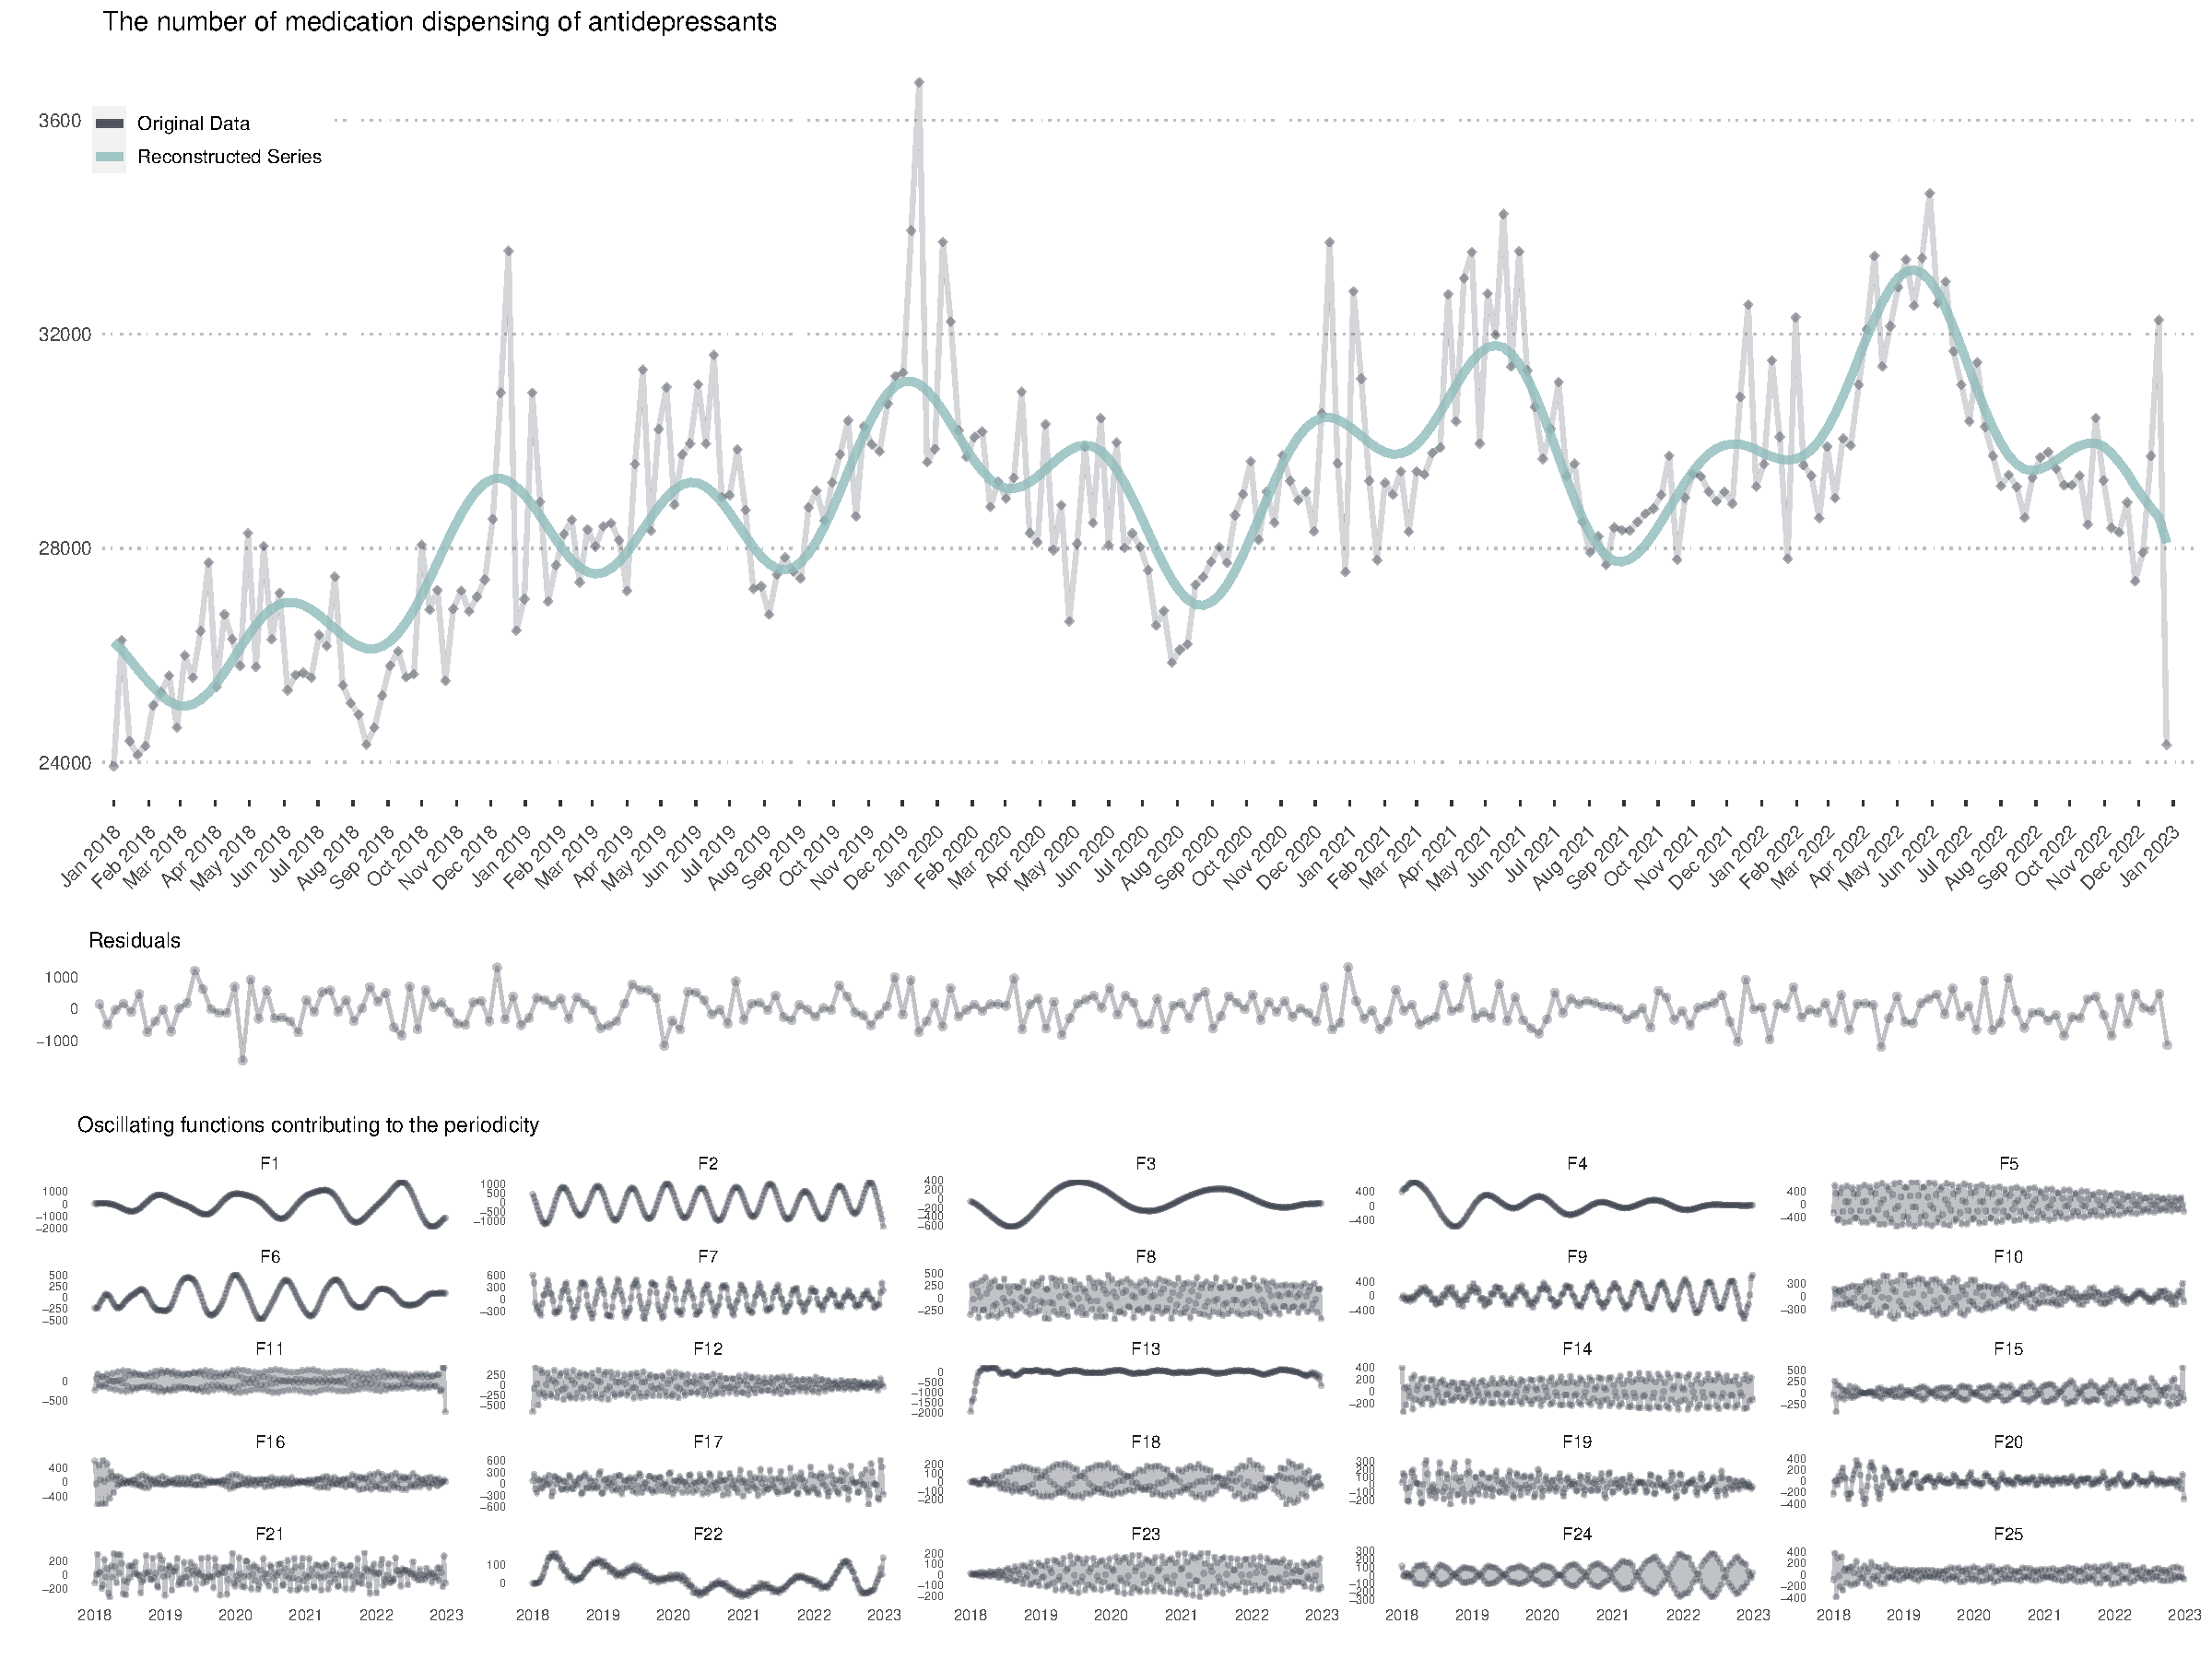
\includegraphics[width=1\linewidth,height=\textheight,keepaspectratio]{article_files/figure-pdf/fig-ssa-1.pdf}

}

\caption{\label{fig-ssa}Time-series decomposition of antidepressants
dispensing data using singular spectrum analysis-based approach}

\end{figure}%

\subsection{Eigenvector centrality
measures}\label{eigenvector-centrality-measures}

Seven medication classes exhibited high centrality, as shown in
Figure~\ref{fig-hi-eigen} and Table~\ref{tbl-desc}. Notably, highly
dispensed medications generally had high eigenvector centrality, which
aligns with the theoretical expectations from
Equation~\ref{eq-eigen-centrality}. However, despite a higher number of
dispensing (6,108,776 vs 5,492,900), antidepressants had lower
eigenvector centrality than medications for the respiratory system
(9.48e-02 {[}SD: 2.24e-03{]} vs 9.53e-02 {[}SD: 2.21e-03{]}). A similar
pattern was observed for anxiolytics, which had more dispensing than
analgesics (2,644,309 vs 2,557,528) but lower eigenvector centrality
(5.25e-02 {[}SD: 4.13e-03{]} vs 5.84e-02 {[}SD: 3.94e-03{]}).

\global\setlength{\Oldarrayrulewidth}{\arrayrulewidth}

\global\setlength{\Oldtabcolsep}{\tabcolsep}

\setlength{\tabcolsep}{0pt}

\renewcommand*{\arraystretch}{1}



\providecommand{\ascline}[3]{\noalign{\global\arrayrulewidth #1}\arrayrulecolor[HTML]{#2}\cline{#3}}

\begin{longtable}[c]{|p{1.57in}|p{0.74in}|p{1.16in}|p{1.16in}|p{1.16in}}

\caption{\label{tbl-desc}Descriptive statistics of dispensing data from
2018 to 2022, ordered by Eigenvector centrality}

\tabularnewline

\ascline{1.5pt}{666666}{1-5}

\multicolumn{2}{>{\centering}m{\dimexpr 2.31in+2\tabcolsep}}{\textcolor[HTML]{000000}{\fontsize{7}{7}\selectfont{\global\setmainfont{DejaVu Sans}{}}}} & \multicolumn{3}{>{\centering}m{\dimexpr 3.49in+4\tabcolsep}}{\textcolor[HTML]{000000}{\fontsize{7}{7}\selectfont{\global\setmainfont{DejaVu Sans}{Mean\ [SD]}}}} \\

\ascline{1.5pt}{666666}{1-5}



\multicolumn{1}{>{\centering}m{\dimexpr 1.57in+0\tabcolsep}}{\textcolor[HTML]{000000}{\fontsize{7}{7}\selectfont{\global\setmainfont{DejaVu Sans}{}}}} & \multicolumn{1}{>{\centering}m{\dimexpr 0.74in+0\tabcolsep}}{\textcolor[HTML]{000000}{\fontsize{7}{7}\selectfont{\global\setmainfont{DejaVu Sans}{Dispensing}}}} & \multicolumn{1}{>{\centering}m{\dimexpr 1.16in+0\tabcolsep}}{\textcolor[HTML]{000000}{\fontsize{7}{7}\selectfont{\global\setmainfont{DejaVu Sans}{Centrality}}}} & \multicolumn{1}{>{\centering}m{\dimexpr 1.16in+0\tabcolsep}}{\textcolor[HTML]{000000}{\fontsize{7}{7}\selectfont{\global\setmainfont{DejaVu Sans}{DDD}}}} & \multicolumn{1}{>{\centering}m{\dimexpr 1.16in+0\tabcolsep}}{\textcolor[HTML]{000000}{\fontsize{7}{7}\selectfont{\global\setmainfont{DejaVu Sans}{Weight}}}} \\

\ascline{1.5pt}{666666}{1-5}\endfirsthead 

\ascline{1.5pt}{666666}{1-5}

\multicolumn{2}{>{\centering}m{\dimexpr 2.31in+2\tabcolsep}}{\textcolor[HTML]{000000}{\fontsize{7}{7}\selectfont{\global\setmainfont{DejaVu Sans}{}}}} & \multicolumn{3}{>{\centering}m{\dimexpr 3.49in+4\tabcolsep}}{\textcolor[HTML]{000000}{\fontsize{7}{7}\selectfont{\global\setmainfont{DejaVu Sans}{Mean\ [SD]}}}} \\

\ascline{1.5pt}{666666}{1-5}



\multicolumn{1}{>{\centering}m{\dimexpr 1.57in+0\tabcolsep}}{\textcolor[HTML]{000000}{\fontsize{7}{7}\selectfont{\global\setmainfont{DejaVu Sans}{}}}} & \multicolumn{1}{>{\centering}m{\dimexpr 0.74in+0\tabcolsep}}{\textcolor[HTML]{000000}{\fontsize{7}{7}\selectfont{\global\setmainfont{DejaVu Sans}{Dispensing}}}} & \multicolumn{1}{>{\centering}m{\dimexpr 1.16in+0\tabcolsep}}{\textcolor[HTML]{000000}{\fontsize{7}{7}\selectfont{\global\setmainfont{DejaVu Sans}{Centrality}}}} & \multicolumn{1}{>{\centering}m{\dimexpr 1.16in+0\tabcolsep}}{\textcolor[HTML]{000000}{\fontsize{7}{7}\selectfont{\global\setmainfont{DejaVu Sans}{DDD}}}} & \multicolumn{1}{>{\centering}m{\dimexpr 1.16in+0\tabcolsep}}{\textcolor[HTML]{000000}{\fontsize{7}{7}\selectfont{\global\setmainfont{DejaVu Sans}{Weight}}}} \\

\ascline{1.5pt}{666666}{1-5}\endhead



\multicolumn{1}{>{\raggedright}m{\dimexpr 1.57in+0\tabcolsep}}{\textcolor[HTML]{000000}{\fontsize{7}{7}\selectfont{\global\setmainfont{DejaVu Sans}{Alimentary\ and\ metabolism}}}} & \multicolumn{1}{>{\centering}m{\dimexpr 0.74in+0\tabcolsep}}{\textcolor[HTML]{000000}{\fontsize{7}{7}\selectfont{\global\setmainfont{DejaVu Sans}{11,512,424}}}} & \multicolumn{1}{>{\centering}m{\dimexpr 1.16in+0\tabcolsep}}{\textcolor[HTML]{000000}{\fontsize{7}{7}\selectfont{\global\setmainfont{DejaVu Sans}{1.59e-01\ [5.00e-03]}}}} & \multicolumn{1}{>{\centering}m{\dimexpr 1.16in+0\tabcolsep}}{\textcolor[HTML]{000000}{\fontsize{7}{7}\selectfont{\global\setmainfont{DejaVu Sans}{5.97e-01\ [3.26e-01]}}}} & \multicolumn{1}{>{\centering}m{\dimexpr 1.16in+0\tabcolsep}}{\textcolor[HTML]{000000}{\fontsize{7}{7}\selectfont{\global\setmainfont{DejaVu Sans}{7.28e-01\ [2.06e-01]}}}} \\





\multicolumn{1}{>{\raggedright}m{\dimexpr 1.57in+0\tabcolsep}}{\textcolor[HTML]{000000}{\fontsize{7}{7}\selectfont{\global\setmainfont{DejaVu Sans}{Cardiovascular}}}} & \multicolumn{1}{>{\centering}m{\dimexpr 0.74in+0\tabcolsep}}{\textcolor[HTML]{000000}{\fontsize{7}{7}\selectfont{\global\setmainfont{DejaVu Sans}{9,778,030}}}} & \multicolumn{1}{>{\centering}m{\dimexpr 1.16in+0\tabcolsep}}{\textcolor[HTML]{000000}{\fontsize{7}{7}\selectfont{\global\setmainfont{DejaVu Sans}{1.50e-01\ [6.87e-03]}}}} & \multicolumn{1}{>{\centering}m{\dimexpr 1.16in+0\tabcolsep}}{\textcolor[HTML]{000000}{\fontsize{7}{7}\selectfont{\global\setmainfont{DejaVu Sans}{5.38e-01\ [3.05e-01]}}}} & \multicolumn{1}{>{\centering}m{\dimexpr 1.16in+0\tabcolsep}}{\textcolor[HTML]{000000}{\fontsize{7}{7}\selectfont{\global\setmainfont{DejaVu Sans}{6.92e-01\ [2.00e-01]}}}} \\





\multicolumn{1}{>{\raggedright}m{\dimexpr 1.57in+0\tabcolsep}}{\textcolor[HTML]{000000}{\fontsize{7}{7}\selectfont{\global\setmainfont{DejaVu Sans}{Respiratory}}}} & \multicolumn{1}{>{\centering}m{\dimexpr 0.74in+0\tabcolsep}}{\textcolor[HTML]{000000}{\fontsize{7}{7}\selectfont{\global\setmainfont{DejaVu Sans}{5,492,900}}}} & \multicolumn{1}{>{\centering}m{\dimexpr 1.16in+0\tabcolsep}}{\textcolor[HTML]{000000}{\fontsize{7}{7}\selectfont{\global\setmainfont{DejaVu Sans}{9.53e-02\ [2.21e-03]}}}} & \multicolumn{1}{>{\centering}m{\dimexpr 1.16in+0\tabcolsep}}{\textcolor[HTML]{000000}{\fontsize{7}{7}\selectfont{\global\setmainfont{DejaVu Sans}{6.55e-01\ [3.25e-01]}}}} & \multicolumn{1}{>{\centering}m{\dimexpr 1.16in+0\tabcolsep}}{\textcolor[HTML]{000000}{\fontsize{7}{7}\selectfont{\global\setmainfont{DejaVu Sans}{7.70e-01\ [2.15e-01]}}}} \\





\multicolumn{1}{>{\raggedright}m{\dimexpr 1.57in+0\tabcolsep}}{\textcolor[HTML]{000000}{\fontsize{7}{7}\selectfont{\global\setmainfont{DejaVu Sans}{Antidepressants}}}} & \multicolumn{1}{>{\centering}m{\dimexpr 0.74in+0\tabcolsep}}{\textcolor[HTML]{000000}{\fontsize{7}{7}\selectfont{\global\setmainfont{DejaVu Sans}{6,108,776}}}} & \multicolumn{1}{>{\centering}m{\dimexpr 1.16in+0\tabcolsep}}{\textcolor[HTML]{000000}{\fontsize{7}{7}\selectfont{\global\setmainfont{DejaVu Sans}{9.48e-02\ [2.24e-03]}}}} & \multicolumn{1}{>{\centering}m{\dimexpr 1.16in+0\tabcolsep}}{\textcolor[HTML]{000000}{\fontsize{7}{7}\selectfont{\global\setmainfont{DejaVu Sans}{5.36e-01\ [3.09e-01]}}}} & \multicolumn{1}{>{\centering}m{\dimexpr 1.16in+0\tabcolsep}}{\textcolor[HTML]{000000}{\fontsize{7}{7}\selectfont{\global\setmainfont{DejaVu Sans}{6.92e-01\ [2.03e-01]}}}} \\





\multicolumn{1}{>{\raggedright}m{\dimexpr 1.57in+0\tabcolsep}}{\textcolor[HTML]{000000}{\fontsize{7}{7}\selectfont{\global\setmainfont{DejaVu Sans}{Blood}}}} & \multicolumn{1}{>{\centering}m{\dimexpr 0.74in+0\tabcolsep}}{\textcolor[HTML]{000000}{\fontsize{7}{7}\selectfont{\global\setmainfont{DejaVu Sans}{2,908,944}}}} & \multicolumn{1}{>{\centering}m{\dimexpr 1.16in+0\tabcolsep}}{\textcolor[HTML]{000000}{\fontsize{7}{7}\selectfont{\global\setmainfont{DejaVu Sans}{8.87e-02\ [5.64e-03]}}}} & \multicolumn{1}{>{\centering}m{\dimexpr 1.16in+0\tabcolsep}}{\textcolor[HTML]{000000}{\fontsize{7}{7}\selectfont{\global\setmainfont{DejaVu Sans}{6.93e-01\ [3.91e-01]}}}} & \multicolumn{1}{>{\centering}m{\dimexpr 1.16in+0\tabcolsep}}{\textcolor[HTML]{000000}{\fontsize{7}{7}\selectfont{\global\setmainfont{DejaVu Sans}{7.78e-01\ [2.13e-01]}}}} \\





\multicolumn{1}{>{\raggedright}m{\dimexpr 1.57in+0\tabcolsep}}{\textcolor[HTML]{000000}{\fontsize{7}{7}\selectfont{\global\setmainfont{DejaVu Sans}{Analgesics}}}} & \multicolumn{1}{>{\centering}m{\dimexpr 0.74in+0\tabcolsep}}{\textcolor[HTML]{000000}{\fontsize{7}{7}\selectfont{\global\setmainfont{DejaVu Sans}{2,557,528}}}} & \multicolumn{1}{>{\centering}m{\dimexpr 1.16in+0\tabcolsep}}{\textcolor[HTML]{000000}{\fontsize{7}{7}\selectfont{\global\setmainfont{DejaVu Sans}{5.84e-02\ [3.94e-03]}}}} & \multicolumn{1}{>{\centering}m{\dimexpr 1.16in+0\tabcolsep}}{\textcolor[HTML]{000000}{\fontsize{7}{7}\selectfont{\global\setmainfont{DejaVu Sans}{4.23e-01\ [2.60e-01]}}}} & \multicolumn{1}{>{\centering}m{\dimexpr 1.16in+0\tabcolsep}}{\textcolor[HTML]{000000}{\fontsize{7}{7}\selectfont{\global\setmainfont{DejaVu Sans}{6.16e-01\ [1.66e-01]}}}} \\





\multicolumn{1}{>{\raggedright}m{\dimexpr 1.57in+0\tabcolsep}}{\textcolor[HTML]{000000}{\fontsize{7}{7}\selectfont{\global\setmainfont{DejaVu Sans}{Anxiolytics}}}} & \multicolumn{1}{>{\centering}m{\dimexpr 0.74in+0\tabcolsep}}{\textcolor[HTML]{000000}{\fontsize{7}{7}\selectfont{\global\setmainfont{DejaVu Sans}{2,644,309}}}} & \multicolumn{1}{>{\centering}m{\dimexpr 1.16in+0\tabcolsep}}{\textcolor[HTML]{000000}{\fontsize{7}{7}\selectfont{\global\setmainfont{DejaVu Sans}{5.25e-02\ [4.13e-03]}}}} & \multicolumn{1}{>{\centering}m{\dimexpr 1.16in+0\tabcolsep}}{\textcolor[HTML]{000000}{\fontsize{7}{7}\selectfont{\global\setmainfont{DejaVu Sans}{4.63e-01\ [2.88e-01]}}}} & \multicolumn{1}{>{\centering}m{\dimexpr 1.16in+0\tabcolsep}}{\textcolor[HTML]{000000}{\fontsize{7}{7}\selectfont{\global\setmainfont{DejaVu Sans}{6.35e-01\ [1.73e-01]}}}} \\





\multicolumn{1}{>{\raggedright}m{\dimexpr 1.57in+0\tabcolsep}}{\textcolor[HTML]{000000}{\fontsize{7}{7}\selectfont{\global\setmainfont{DejaVu Sans}{Dermatologicals}}}} & \multicolumn{1}{>{\centering}m{\dimexpr 0.74in+0\tabcolsep}}{\textcolor[HTML]{000000}{\fontsize{7}{7}\selectfont{\global\setmainfont{DejaVu Sans}{2,086,095}}}} & \multicolumn{1}{>{\centering}m{\dimexpr 1.16in+0\tabcolsep}}{\textcolor[HTML]{000000}{\fontsize{7}{7}\selectfont{\global\setmainfont{DejaVu Sans}{4.03e-02\ [1.34e-03]}}}} & \multicolumn{1}{>{\centering}m{\dimexpr 1.16in+0\tabcolsep}}{\textcolor[HTML]{000000}{\fontsize{7}{7}\selectfont{\global\setmainfont{DejaVu Sans}{8.08e-01\ [3.39e-01]}}}} & \multicolumn{1}{>{\centering}m{\dimexpr 1.16in+0\tabcolsep}}{\textcolor[HTML]{000000}{\fontsize{7}{7}\selectfont{\global\setmainfont{DejaVu Sans}{8.62e-01\ [2.09e-01]}}}} \\





\multicolumn{1}{>{\raggedright}m{\dimexpr 1.57in+0\tabcolsep}}{\textcolor[HTML]{000000}{\fontsize{7}{7}\selectfont{\global\setmainfont{DejaVu Sans}{Musculoskeletal}}}} & \multicolumn{1}{>{\centering}m{\dimexpr 0.74in+0\tabcolsep}}{\textcolor[HTML]{000000}{\fontsize{7}{7}\selectfont{\global\setmainfont{DejaVu Sans}{1,449,535}}}} & \multicolumn{1}{>{\centering}m{\dimexpr 1.16in+0\tabcolsep}}{\textcolor[HTML]{000000}{\fontsize{7}{7}\selectfont{\global\setmainfont{DejaVu Sans}{3.95e-02\ [1.52e-03]}}}} & \multicolumn{1}{>{\centering}m{\dimexpr 1.16in+0\tabcolsep}}{\textcolor[HTML]{000000}{\fontsize{7}{7}\selectfont{\global\setmainfont{DejaVu Sans}{5.59e-01\ [3.26e-01]}}}} & \multicolumn{1}{>{\centering}m{\dimexpr 1.16in+0\tabcolsep}}{\textcolor[HTML]{000000}{\fontsize{7}{7}\selectfont{\global\setmainfont{DejaVu Sans}{7.10e-01\ [2.11e-01]}}}} \\





\multicolumn{1}{>{\raggedright}m{\dimexpr 1.57in+0\tabcolsep}}{\textcolor[HTML]{000000}{\fontsize{7}{7}\selectfont{\global\setmainfont{DejaVu Sans}{Systemic\ hormonal}}}} & \multicolumn{1}{>{\centering}m{\dimexpr 0.74in+0\tabcolsep}}{\textcolor[HTML]{000000}{\fontsize{7}{7}\selectfont{\global\setmainfont{DejaVu Sans}{1,602,716}}}} & \multicolumn{1}{>{\centering}m{\dimexpr 1.16in+0\tabcolsep}}{\textcolor[HTML]{000000}{\fontsize{7}{7}\selectfont{\global\setmainfont{DejaVu Sans}{3.80e-02\ [1.71e-03]}}}} & \multicolumn{1}{>{\centering}m{\dimexpr 1.16in+0\tabcolsep}}{\textcolor[HTML]{000000}{\fontsize{7}{7}\selectfont{\global\setmainfont{DejaVu Sans}{4.97e-01\ [2.76e-01]}}}} & \multicolumn{1}{>{\centering}m{\dimexpr 1.16in+0\tabcolsep}}{\textcolor[HTML]{000000}{\fontsize{7}{7}\selectfont{\global\setmainfont{DejaVu Sans}{6.55e-01\ [1.66e-01]}}}} \\





\multicolumn{1}{>{\raggedright}m{\dimexpr 1.57in+0\tabcolsep}}{\textcolor[HTML]{000000}{\fontsize{7}{7}\selectfont{\global\setmainfont{DejaVu Sans}{Antipsychotics}}}} & \multicolumn{1}{>{\centering}m{\dimexpr 0.74in+0\tabcolsep}}{\textcolor[HTML]{000000}{\fontsize{7}{7}\selectfont{\global\setmainfont{DejaVu Sans}{2,473,609}}}} & \multicolumn{1}{>{\centering}m{\dimexpr 1.16in+0\tabcolsep}}{\textcolor[HTML]{000000}{\fontsize{7}{7}\selectfont{\global\setmainfont{DejaVu Sans}{3.70e-02\ [3.20e-03]}}}} & \multicolumn{1}{>{\centering}m{\dimexpr 1.16in+0\tabcolsep}}{\textcolor[HTML]{000000}{\fontsize{7}{7}\selectfont{\global\setmainfont{DejaVu Sans}{4.04e-01\ [2.65e-01]}}}} & \multicolumn{1}{>{\centering}m{\dimexpr 1.16in+0\tabcolsep}}{\textcolor[HTML]{000000}{\fontsize{7}{7}\selectfont{\global\setmainfont{DejaVu Sans}{6.10e-01\ [1.69e-01]}}}} \\





\multicolumn{1}{>{\raggedright}m{\dimexpr 1.57in+0\tabcolsep}}{\textcolor[HTML]{000000}{\fontsize{7}{7}\selectfont{\global\setmainfont{DejaVu Sans}{Genitourinary}}}} & \multicolumn{1}{>{\centering}m{\dimexpr 0.74in+0\tabcolsep}}{\textcolor[HTML]{000000}{\fontsize{7}{7}\selectfont{\global\setmainfont{DejaVu Sans}{2,099,833}}}} & \multicolumn{1}{>{\centering}m{\dimexpr 1.16in+0\tabcolsep}}{\textcolor[HTML]{000000}{\fontsize{7}{7}\selectfont{\global\setmainfont{DejaVu Sans}{3.39e-02\ [9.53e-04]}}}} & \multicolumn{1}{>{\centering}m{\dimexpr 1.16in+0\tabcolsep}}{\textcolor[HTML]{000000}{\fontsize{7}{7}\selectfont{\global\setmainfont{DejaVu Sans}{7.46e-01\ [3.69e-01]}}}} & \multicolumn{1}{>{\centering}m{\dimexpr 1.16in+0\tabcolsep}}{\textcolor[HTML]{000000}{\fontsize{7}{7}\selectfont{\global\setmainfont{DejaVu Sans}{8.29e-01\ [2.12e-01]}}}} \\





\multicolumn{1}{>{\raggedright}m{\dimexpr 1.57in+0\tabcolsep}}{\textcolor[HTML]{000000}{\fontsize{7}{7}\selectfont{\global\setmainfont{DejaVu Sans}{Hypnotics\ and\ sedatives}}}} & \multicolumn{1}{>{\centering}m{\dimexpr 0.74in+0\tabcolsep}}{\textcolor[HTML]{000000}{\fontsize{7}{7}\selectfont{\global\setmainfont{DejaVu Sans}{1,467,752}}}} & \multicolumn{1}{>{\centering}m{\dimexpr 1.16in+0\tabcolsep}}{\textcolor[HTML]{000000}{\fontsize{7}{7}\selectfont{\global\setmainfont{DejaVu Sans}{3.37e-02\ [3.23e-03]}}}} & \multicolumn{1}{>{\centering}m{\dimexpr 1.16in+0\tabcolsep}}{\textcolor[HTML]{000000}{\fontsize{7}{7}\selectfont{\global\setmainfont{DejaVu Sans}{6.31e-01\ [3.16e-01]}}}} & \multicolumn{1}{>{\centering}m{\dimexpr 1.16in+0\tabcolsep}}{\textcolor[HTML]{000000}{\fontsize{7}{7}\selectfont{\global\setmainfont{DejaVu Sans}{7.49e-01\ [2.09e-01]}}}} \\





\multicolumn{1}{>{\raggedright}m{\dimexpr 1.57in+0\tabcolsep}}{\textcolor[HTML]{000000}{\fontsize{7}{7}\selectfont{\global\setmainfont{DejaVu Sans}{Systemic\ anti-infectives}}}} & \multicolumn{1}{>{\centering}m{\dimexpr 0.74in+0\tabcolsep}}{\textcolor[HTML]{000000}{\fontsize{7}{7}\selectfont{\global\setmainfont{DejaVu Sans}{734,706}}}} & \multicolumn{1}{>{\centering}m{\dimexpr 1.16in+0\tabcolsep}}{\textcolor[HTML]{000000}{\fontsize{7}{7}\selectfont{\global\setmainfont{DejaVu Sans}{2.07e-02\ [1.47e-03]}}}} & \multicolumn{1}{>{\centering}m{\dimexpr 1.16in+0\tabcolsep}}{\textcolor[HTML]{000000}{\fontsize{7}{7}\selectfont{\global\setmainfont{DejaVu Sans}{6.34e-01\ [3.23e-01]}}}} & \multicolumn{1}{>{\centering}m{\dimexpr 1.16in+0\tabcolsep}}{\textcolor[HTML]{000000}{\fontsize{7}{7}\selectfont{\global\setmainfont{DejaVu Sans}{7.64e-01\ [2.21e-01]}}}} \\





\multicolumn{1}{>{\raggedright}m{\dimexpr 1.57in+0\tabcolsep}}{\textcolor[HTML]{000000}{\fontsize{7}{7}\selectfont{\global\setmainfont{DejaVu Sans}{Antiepileptics}}}} & \multicolumn{1}{>{\centering}m{\dimexpr 0.74in+0\tabcolsep}}{\textcolor[HTML]{000000}{\fontsize{7}{7}\selectfont{\global\setmainfont{DejaVu Sans}{1,078,266}}}} & \multicolumn{1}{>{\centering}m{\dimexpr 1.16in+0\tabcolsep}}{\textcolor[HTML]{000000}{\fontsize{7}{7}\selectfont{\global\setmainfont{DejaVu Sans}{2.06e-02\ [2.73e-03]}}}} & \multicolumn{1}{>{\centering}m{\dimexpr 1.16in+0\tabcolsep}}{\textcolor[HTML]{000000}{\fontsize{7}{7}\selectfont{\global\setmainfont{DejaVu Sans}{4.29e-01\ [2.52e-01]}}}} & \multicolumn{1}{>{\centering}m{\dimexpr 1.16in+0\tabcolsep}}{\textcolor[HTML]{000000}{\fontsize{7}{7}\selectfont{\global\setmainfont{DejaVu Sans}{6.25e-01\ [1.66e-01]}}}} \\





\multicolumn{1}{>{\raggedright}m{\dimexpr 1.57in+0\tabcolsep}}{\textcolor[HTML]{000000}{\fontsize{7}{7}\selectfont{\global\setmainfont{DejaVu Sans}{Antineoplastics}}}} & \multicolumn{1}{>{\centering}m{\dimexpr 0.74in+0\tabcolsep}}{\textcolor[HTML]{000000}{\fontsize{7}{7}\selectfont{\global\setmainfont{DejaVu Sans}{449,030}}}} & \multicolumn{1}{>{\centering}m{\dimexpr 1.16in+0\tabcolsep}}{\textcolor[HTML]{000000}{\fontsize{7}{7}\selectfont{\global\setmainfont{DejaVu Sans}{1.03e-02\ [4.68e-04]}}}} & \multicolumn{1}{>{\centering}m{\dimexpr 1.16in+0\tabcolsep}}{\textcolor[HTML]{000000}{\fontsize{7}{7}\selectfont{\global\setmainfont{DejaVu Sans}{6.13e-01\ [3.01e-01]}}}} & \multicolumn{1}{>{\centering}m{\dimexpr 1.16in+0\tabcolsep}}{\textcolor[HTML]{000000}{\fontsize{7}{7}\selectfont{\global\setmainfont{DejaVu Sans}{7.49e-01\ [2.05e-01]}}}} \\





\multicolumn{1}{>{\raggedright}m{\dimexpr 1.57in+0\tabcolsep}}{\textcolor[HTML]{000000}{\fontsize{7}{7}\selectfont{\global\setmainfont{DejaVu Sans}{Other\ nervous\ system\ drugs}}}} & \multicolumn{1}{>{\centering}m{\dimexpr 0.74in+0\tabcolsep}}{\textcolor[HTML]{000000}{\fontsize{7}{7}\selectfont{\global\setmainfont{DejaVu Sans}{362,624}}}} & \multicolumn{1}{>{\centering}m{\dimexpr 1.16in+0\tabcolsep}}{\textcolor[HTML]{000000}{\fontsize{7}{7}\selectfont{\global\setmainfont{DejaVu Sans}{8.79e-03\ [1.08e-03]}}}} & \multicolumn{1}{>{\centering}m{\dimexpr 1.16in+0\tabcolsep}}{\textcolor[HTML]{000000}{\fontsize{7}{7}\selectfont{\global\setmainfont{DejaVu Sans}{5.23e-01\ [3.16e-01]}}}} & \multicolumn{1}{>{\centering}m{\dimexpr 1.16in+0\tabcolsep}}{\textcolor[HTML]{000000}{\fontsize{7}{7}\selectfont{\global\setmainfont{DejaVu Sans}{6.78e-01\ [1.93e-01]}}}} \\





\multicolumn{1}{>{\raggedright}m{\dimexpr 1.57in+0\tabcolsep}}{\textcolor[HTML]{000000}{\fontsize{7}{7}\selectfont{\global\setmainfont{DejaVu Sans}{Antiparkinson}}}} & \multicolumn{1}{>{\centering}m{\dimexpr 0.74in+0\tabcolsep}}{\textcolor[HTML]{000000}{\fontsize{7}{7}\selectfont{\global\setmainfont{DejaVu Sans}{306,541}}}} & \multicolumn{1}{>{\centering}m{\dimexpr 1.16in+0\tabcolsep}}{\textcolor[HTML]{000000}{\fontsize{7}{7}\selectfont{\global\setmainfont{DejaVu Sans}{6.17e-03\ [5.64e-04]}}}} & \multicolumn{1}{>{\centering}m{\dimexpr 1.16in+0\tabcolsep}}{\textcolor[HTML]{000000}{\fontsize{7}{7}\selectfont{\global\setmainfont{DejaVu Sans}{3.53e-01\ [2.21e-01]}}}} & \multicolumn{1}{>{\centering}m{\dimexpr 1.16in+0\tabcolsep}}{\textcolor[HTML]{000000}{\fontsize{7}{7}\selectfont{\global\setmainfont{DejaVu Sans}{5.74e-01\ [1.37e-01]}}}} \\





\multicolumn{1}{>{\raggedright}m{\dimexpr 1.57in+0\tabcolsep}}{\textcolor[HTML]{000000}{\fontsize{7}{7}\selectfont{\global\setmainfont{DejaVu Sans}{Psychostimulants}}}} & \multicolumn{1}{>{\centering}m{\dimexpr 0.74in+0\tabcolsep}}{\textcolor[HTML]{000000}{\fontsize{7}{7}\selectfont{\global\setmainfont{DejaVu Sans}{459,207}}}} & \multicolumn{1}{>{\centering}m{\dimexpr 1.16in+0\tabcolsep}}{\textcolor[HTML]{000000}{\fontsize{7}{7}\selectfont{\global\setmainfont{DejaVu Sans}{5.56e-03\ [8.26e-04]}}}} & \multicolumn{1}{>{\centering}m{\dimexpr 1.16in+0\tabcolsep}}{\textcolor[HTML]{000000}{\fontsize{7}{7}\selectfont{\global\setmainfont{DejaVu Sans}{5.20e-01\ [3.13e-01]}}}} & \multicolumn{1}{>{\centering}m{\dimexpr 1.16in+0\tabcolsep}}{\textcolor[HTML]{000000}{\fontsize{7}{7}\selectfont{\global\setmainfont{DejaVu Sans}{6.74e-01\ [1.90e-01]}}}} \\





\multicolumn{1}{>{\raggedright}m{\dimexpr 1.57in+0\tabcolsep}}{\textcolor[HTML]{000000}{\fontsize{7}{7}\selectfont{\global\setmainfont{DejaVu Sans}{Sensory}}}} & \multicolumn{1}{>{\centering}m{\dimexpr 0.74in+0\tabcolsep}}{\textcolor[HTML]{000000}{\fontsize{7}{7}\selectfont{\global\setmainfont{DejaVu Sans}{196,513}}}} & \multicolumn{1}{>{\centering}m{\dimexpr 1.16in+0\tabcolsep}}{\textcolor[HTML]{000000}{\fontsize{7}{7}\selectfont{\global\setmainfont{DejaVu Sans}{3.36e-03\ [5.91e-04]}}}} & \multicolumn{1}{>{\centering}m{\dimexpr 1.16in+0\tabcolsep}}{\textcolor[HTML]{000000}{\fontsize{7}{7}\selectfont{\global\setmainfont{DejaVu Sans}{4.66e-01\ [2.87e-01]}}}} & \multicolumn{1}{>{\centering}m{\dimexpr 1.16in+0\tabcolsep}}{\textcolor[HTML]{000000}{\fontsize{7}{7}\selectfont{\global\setmainfont{DejaVu Sans}{6.37e-01\ [1.80e-01]}}}} \\





\multicolumn{1}{>{\raggedright}m{\dimexpr 1.57in+0\tabcolsep}}{\textcolor[HTML]{000000}{\fontsize{7}{7}\selectfont{\global\setmainfont{DejaVu Sans}{Antiparasitics}}}} & \multicolumn{1}{>{\centering}m{\dimexpr 0.74in+0\tabcolsep}}{\textcolor[HTML]{000000}{\fontsize{7}{7}\selectfont{\global\setmainfont{DejaVu Sans}{88,760}}}} & \multicolumn{1}{>{\centering}m{\dimexpr 1.16in+0\tabcolsep}}{\textcolor[HTML]{000000}{\fontsize{7}{7}\selectfont{\global\setmainfont{DejaVu Sans}{1.61e-03\ [1.20e-04]}}}} & \multicolumn{1}{>{\centering}m{\dimexpr 1.16in+0\tabcolsep}}{\textcolor[HTML]{000000}{\fontsize{7}{7}\selectfont{\global\setmainfont{DejaVu Sans}{5.24e-01\ [2.53e-01]}}}} & \multicolumn{1}{>{\centering}m{\dimexpr 1.16in+0\tabcolsep}}{\textcolor[HTML]{000000}{\fontsize{7}{7}\selectfont{\global\setmainfont{DejaVu Sans}{6.72e-01\ [1.65e-01]}}}} \\





\multicolumn{1}{>{\raggedright}m{\dimexpr 1.57in+0\tabcolsep}}{\textcolor[HTML]{000000}{\fontsize{7}{7}\selectfont{\global\setmainfont{DejaVu Sans}{Anesthetic}}}} & \multicolumn{1}{>{\centering}m{\dimexpr 0.74in+0\tabcolsep}}{\textcolor[HTML]{000000}{\fontsize{7}{7}\selectfont{\global\setmainfont{DejaVu Sans}{39,455}}}} & \multicolumn{1}{>{\centering}m{\dimexpr 1.16in+0\tabcolsep}}{\textcolor[HTML]{000000}{\fontsize{7}{7}\selectfont{\global\setmainfont{DejaVu Sans}{1.15e-03\ [2.15e-04]}}}} & \multicolumn{1}{>{\centering}m{\dimexpr 1.16in+0\tabcolsep}}{\textcolor[HTML]{000000}{\fontsize{7}{7}\selectfont{\global\setmainfont{DejaVu Sans}{6.45e-01\ [4.47e-01]}}}} & \multicolumn{1}{>{\centering}m{\dimexpr 1.16in+0\tabcolsep}}{\textcolor[HTML]{000000}{\fontsize{7}{7}\selectfont{\global\setmainfont{DejaVu Sans}{7.39e-01\ [2.31e-01]}}}} \\





\multicolumn{1}{>{\raggedright}m{\dimexpr 1.57in+0\tabcolsep}}{\textcolor[HTML]{000000}{\fontsize{7}{7}\selectfont{\global\setmainfont{DejaVu Sans}{Others}}}} & \multicolumn{1}{>{\centering}m{\dimexpr 0.74in+0\tabcolsep}}{\textcolor[HTML]{000000}{\fontsize{7}{7}\selectfont{\global\setmainfont{DejaVu Sans}{18,157}}}} & \multicolumn{1}{>{\centering}m{\dimexpr 1.16in+0\tabcolsep}}{\textcolor[HTML]{000000}{\fontsize{7}{7}\selectfont{\global\setmainfont{DejaVu Sans}{2.94e-04\ [4.86e-05]}}}} & \multicolumn{1}{>{\centering}m{\dimexpr 1.16in+0\tabcolsep}}{\textcolor[HTML]{000000}{\fontsize{7}{7}\selectfont{\global\setmainfont{DejaVu Sans}{4.55e-01\ [2.73e-01]}}}} & \multicolumn{1}{>{\centering}m{\dimexpr 1.16in+0\tabcolsep}}{\textcolor[HTML]{000000}{\fontsize{7}{7}\selectfont{\global\setmainfont{DejaVu Sans}{6.37e-01\ [1.77e-01]}}}} \\





\multicolumn{1}{>{\raggedright}m{\dimexpr 1.57in+0\tabcolsep}}{\textcolor[HTML]{000000}{\fontsize{7}{7}\selectfont{\global\setmainfont{DejaVu Sans}{Antidementia}}}} & \multicolumn{1}{>{\centering}m{\dimexpr 0.74in+0\tabcolsep}}{\textcolor[HTML]{000000}{\fontsize{7}{7}\selectfont{\global\setmainfont{DejaVu Sans}{9,937}}}} & \multicolumn{1}{>{\centering}m{\dimexpr 1.16in+0\tabcolsep}}{\textcolor[HTML]{000000}{\fontsize{7}{7}\selectfont{\global\setmainfont{DejaVu Sans}{2.00e-04\ [4.76e-05]}}}} & \multicolumn{1}{>{\centering}m{\dimexpr 1.16in+0\tabcolsep}}{\textcolor[HTML]{000000}{\fontsize{7}{7}\selectfont{\global\setmainfont{DejaVu Sans}{6.80e-01\ [2.85e-01]}}}} & \multicolumn{1}{>{\centering}m{\dimexpr 1.16in+0\tabcolsep}}{\textcolor[HTML]{000000}{\fontsize{7}{7}\selectfont{\global\setmainfont{DejaVu Sans}{7.87e-01\ [2.02e-01]}}}} \\

\ascline{1.5pt}{666666}{1-5}


\end{longtable}

\arrayrulecolor[HTML]{000000}

\global\setlength{\arrayrulewidth}{\Oldarrayrulewidth}

\global\setlength{\tabcolsep}{\Oldtabcolsep}

\renewcommand*{\arraystretch}{1}

\begin{figure}

\centering{

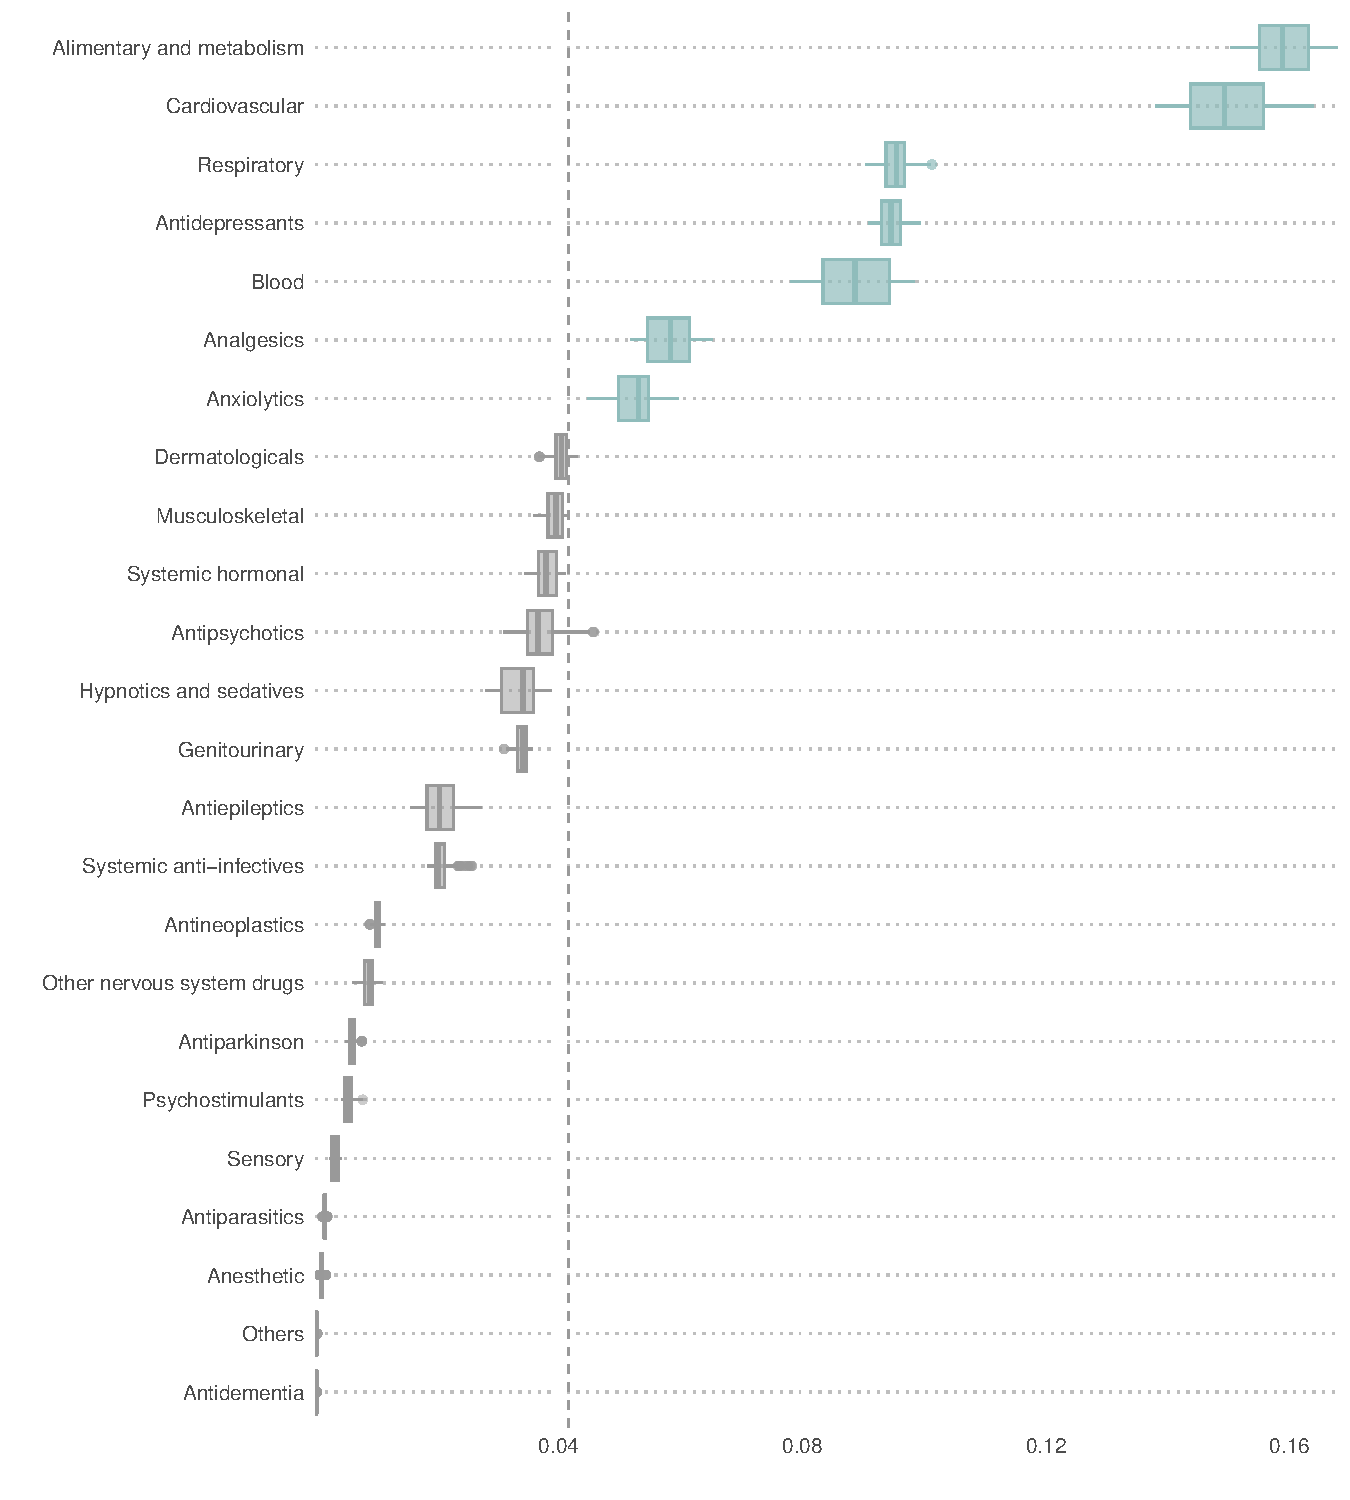
\includegraphics[width=1\linewidth,height=\textheight,keepaspectratio]{article_files/figure-pdf/fig-hi-eigen-1.pdf}

}

\caption{\label{fig-hi-eigen}Clusters of medication with a significant
influence on how antidepressants and anxiolytics are prescribed}

\end{figure}%

\section{Discussion}\label{discussion}

This network analysis of dispensing data in individuals using
antidepressants or anxiolytics revealed distinct polypharmacy patterns
between these groups. While same-class polypharmacy was more common
among antidepressant users, multi-class polypharmacy predominated among
those receiving anxiolytics. Notably, in both groups, multi-class
polypharmacy was at least ten times more prevalent than same-class
polypharmacy. Seven medication classes exhibited high eigenvector
centrality, indicating their strong influence on co-prescription
dynamics. These include medications for the alimentary tract and
metabolism (ATC code \texttt{A}), blood and blood-forming organs
(\texttt{B}), cardiovascular system (\texttt{C}), respiratory system
(\texttt{R}), and analgesics (\texttt{N02}). These classes do not merely
appear frequently but also serve as key connectors within prescribing
networks, linking psychiatric treatments to chronic disease management.
Their centrality suggests that they play a role in structuring
multi-class polypharmacy, either as standard co-prescriptions due to
clinical guidelines or as necessary adjuncts in managing comorbidities.

Our findings align with previous research showing that antidepressants
and anxiolytics are frequently co-prescribed with other medications
\citep{Shrivastava2013}, and that multi-class regimens contribute most
to psychopharmaca polypharmacy \citep{de2004polypharmacy}. Furthermore,
there have been established bidirectional associations between
depression/anxiety and chronic illnesses \citep{qi2024longitudinal}.
Conditions such as diabetes mellitus, thyroid disorders, and asthma have
been linked to an increased risk of depression \citep{jang2024temporal}.
The need for long-term pharmacological management further drives
co-prescription patterns. Additionally, chronic illness-related anxiety
can contribute to heightened prescribing of anxiolytics
\citep{lebel2020health}. This underscores the interconnected nature of
psychopharmaca prescribing patterns and highlights the complexity of
medication management in these populations.

DPN complements traditional drug utilization analyses by capturing the
structural properties of prescribing behaviors. Beyond evaluating
individual drug utilization or basic pairwise co-prescriptions, DPN
provides a structural perspective by mapping the interconnections
between medications within a broader prescribing network
\citep{Bazzoni2015}. The network approach is a particularly useful
method for understanding complex prescribing dynamics, which allows for
the identification of central medication classes that influence
polypharmacy patterns. The high centrality of certain medication classes
suggests they serve as critical connectors in treatment regimens,
providing the basis for further monitoring and evaluation.

By mapping the relationships between medications, DPN enables the
detection of patterns that would be challenging to observe through
standard statistical methods. For instance, the high centrality of
certain medication classes suggests that they play a pivotal role in
multi-class polypharmacy, likely due to their involvement in managing
both psychiatric and non-psychiatric conditions. As such, network
analysis is a suitable approach for generating hypothesis, which has
also been thoroughly discussed by \citet{Askar2021}.

We acknowledge several limitations in this study. First, data
aggregation at the population level resulted in the loss of
individual-level information, limiting interpretation to population
trends. Second, while the adjustment of weights based on DDD introduces
a novel element to the analysis, it is important to note that DDD values
are not always equal to one, as defined by the WHO ATC system. Our study
adopted a DDD-based weighting approach to refine network edges, aligning
with the recommendation of \citet{Cavallo2012}. The adjusted weighting
penalizes values deviating significantly from 1, reducing their impact
on the network. Future research should explore alternative weighting
techniques, such as patient-level dosage adjustments, to enhance network
precision.

Despite the limitations, our study demonstrates the utility of DPN as a
powerful, data-driven approach to analyzing medication dispensing data.
By modelling intricate co-prescription patterns, DPN filters medication
classes based on network properties, offering insights into prescribing
behaviors. These insights can reveal important trends in medication use,
which can be useful to public health monitoring. By capturing the
complexity of drug prescription relationships, DPN holds significant
potential to improve decision-making in both clinical and administrative
contexts.

Future DPN studies on individuals using antidepressants or anxiolytics
should adopt a more fine-grained ATC classification to identify specific
medications driving polypharmacy patterns within the currently
identified seven medication classes. A more granular approach could
reveal whether certain drugs disproportionately contribute to
multi-class polypharmacy and whether these prescribing trends vary
across patient demographics or healthcare settings. Such insights could
refine our understanding of prescribing behaviors and inform targeted
interventions for optimizing medication regimens.

\section{Conclusion}\label{conclusion}

This study utilized DPN to evaluate the influence of specific medication
classes on prescribing patterns of antidepressants and anxiolytics. By
focusing on co-prescription patterns, we identified seven medication
classes with significant eigenvector centrality, reflecting their
critical role in polypharmacy regimens for individuals using anxiolytics
and antidepressants. This study highlights the potential of
network-based approaches to narrow down high-impact medications for
further evaluation.


\renewcommand\refname{References}
  \bibliography{ref.bib}



\end{document}
